\documentclass[12pt]{article}
\usepackage[utf8]{inputenc}
\usepackage{graphicx}
\usepackage{amsmath}
\usepackage{booktabs}
\usepackage{geometry}
\usepackage{hyperref}
\usepackage{titlesec}
\usepackage{float}
\usepackage{lipsum}

\geometry{letterpaper, margin=0.75in}
\hypersetup{colorlinks=true, linkcolor=blue, filecolor=magenta, urlcolor=cyan}

\begin{document}

\begin{titlepage}
    \centering
    \vspace*{2cm}
    {\huge \textbf{Design and Implementation of High-Throughput 175-Tap FIR Filter Architectures} \par}
    \vspace{1.5cm}
    {\Large Jaden Tompkins \par}
    \vspace{0.5cm}
    {\large Advanced VLSI Design (ECSE 6680) \par}
    {\large Rensselaer Polytechnic Institute \par}
    \vfill
    {\large \today \par}
\end{titlepage}

\newpage

\begin{abstract}
This report presents a comprehensive design space exploration of 175-tap FIR filter architectures. By analyzing performance metrics such as area (ALMs), power, and $F_{max}$ for seven distinct designs, we demonstrate the throughput advantages of parallel and pipelined structures.
\end{abstract}

\section{Introduction}
FIR filters are fundamental blocks in digital communications and signal processing, where high-throughput and area-efficiency are primary design constraints. This project explores the end-to-end design space for a 175-tap FIR filter, from algorithm development in MATLAB to high-speed hardware implementation on an FPGA. The following specifications were provided as initial project guidelines:
\begin{itemize}
    \item Low pass FIR filter
    \item Suggested 100 taps
    \item 80dB stopband attenuation
    \item $0.2\pi$ to $0.23\pi$ transition band
\end{itemize}
From here, MATLAB was used to find the minimum filter order required to meet the specifications:
\begin{itemize}
    \item 175 taps
    \item 16-bit inputs
    \item 24-bit coefficients
    \item 49-bit accumulators
    \item 23 fractional bits
    \item 16-bit outputs
\end{itemize}
This MATLAB "golden reference" was used to generate the coefficients and test vectors for the hardware implementations. The following architectures were implemented:
\begin{itemize}
    \item Direct Form - Baseline
    \item Pipelined Direct Form - Filtering broken into stages
    \item Parallel L=2 - Polyphase decomposition with 2 parallel sub-filters
    \item Fast FIR L=2 - Parallel (L=2) architecture following Fast FIR Algorithm
    \item Parallel L=3 - Polyphase decomposition with 3 parallel sub-filters
    \item Fast FIR L=3 - Parallel (L=3) architecture following Fast FIR Algorithm
    \item Pipelined Fast FIR L=3 - Parallel (L=3) architecture following Fast FIR Algorithm and pipelining
\end{itemize}
FFA speeds up the filter by reducing the total number of sub-filter modules required to process multiple samples in parallel. This algorithmic optimization lowers the hardware complexity and power consumption compared to traditional brute-force parallel implementations, allowing for high-throughput designs with a significantly reduced resource footprint. Through this comprehensive design space exploration, the Pipelined Fast FIR $L=3$ architecture was identified as the optimal design, providing a 6x throughput increase over the baseline with minimal resource overhead.

\section{MATLAB Design Methodology}
The filter design phase utilizes MATLAB as the golden reference for coefficient generation, fixed-point analysis, and automated hardware integration. This ensures that the hardware implementation precisely matches the theoretical performance requirements through a systematic, reproducible workflow.

\subsection{Filter Specification and Iterative Design}
The design targets a high-order low-pass FIR filter using the Parks-McClellan Remez exchange algorithm (\texttt{firpm}). An automated design script was developed to iteratively determine the minimum filter order required to meet the stringent 80dB stopband attenuation requirement. Starting from a baseline of 100 taps, the script increases the order until the peak stopband ripple falls below the threshold, resulting in a 175-tap equiripple design. 

The filter specifications used across all architectural explorations are as follows:
\begin{itemize}
    \item \textbf{Type:} Low-Pass Equiripple (Parks-McClellan)
    \item \textbf{Taps:} 175
    \item \textbf{Transition Band:} 0.2$\pi$ to 0.23$\pi$ rad/sample
    \item \textbf{Stopband Attenuation:} $>$ 80 dB
\end{itemize}

\begin{figure}[H]
    \centering
    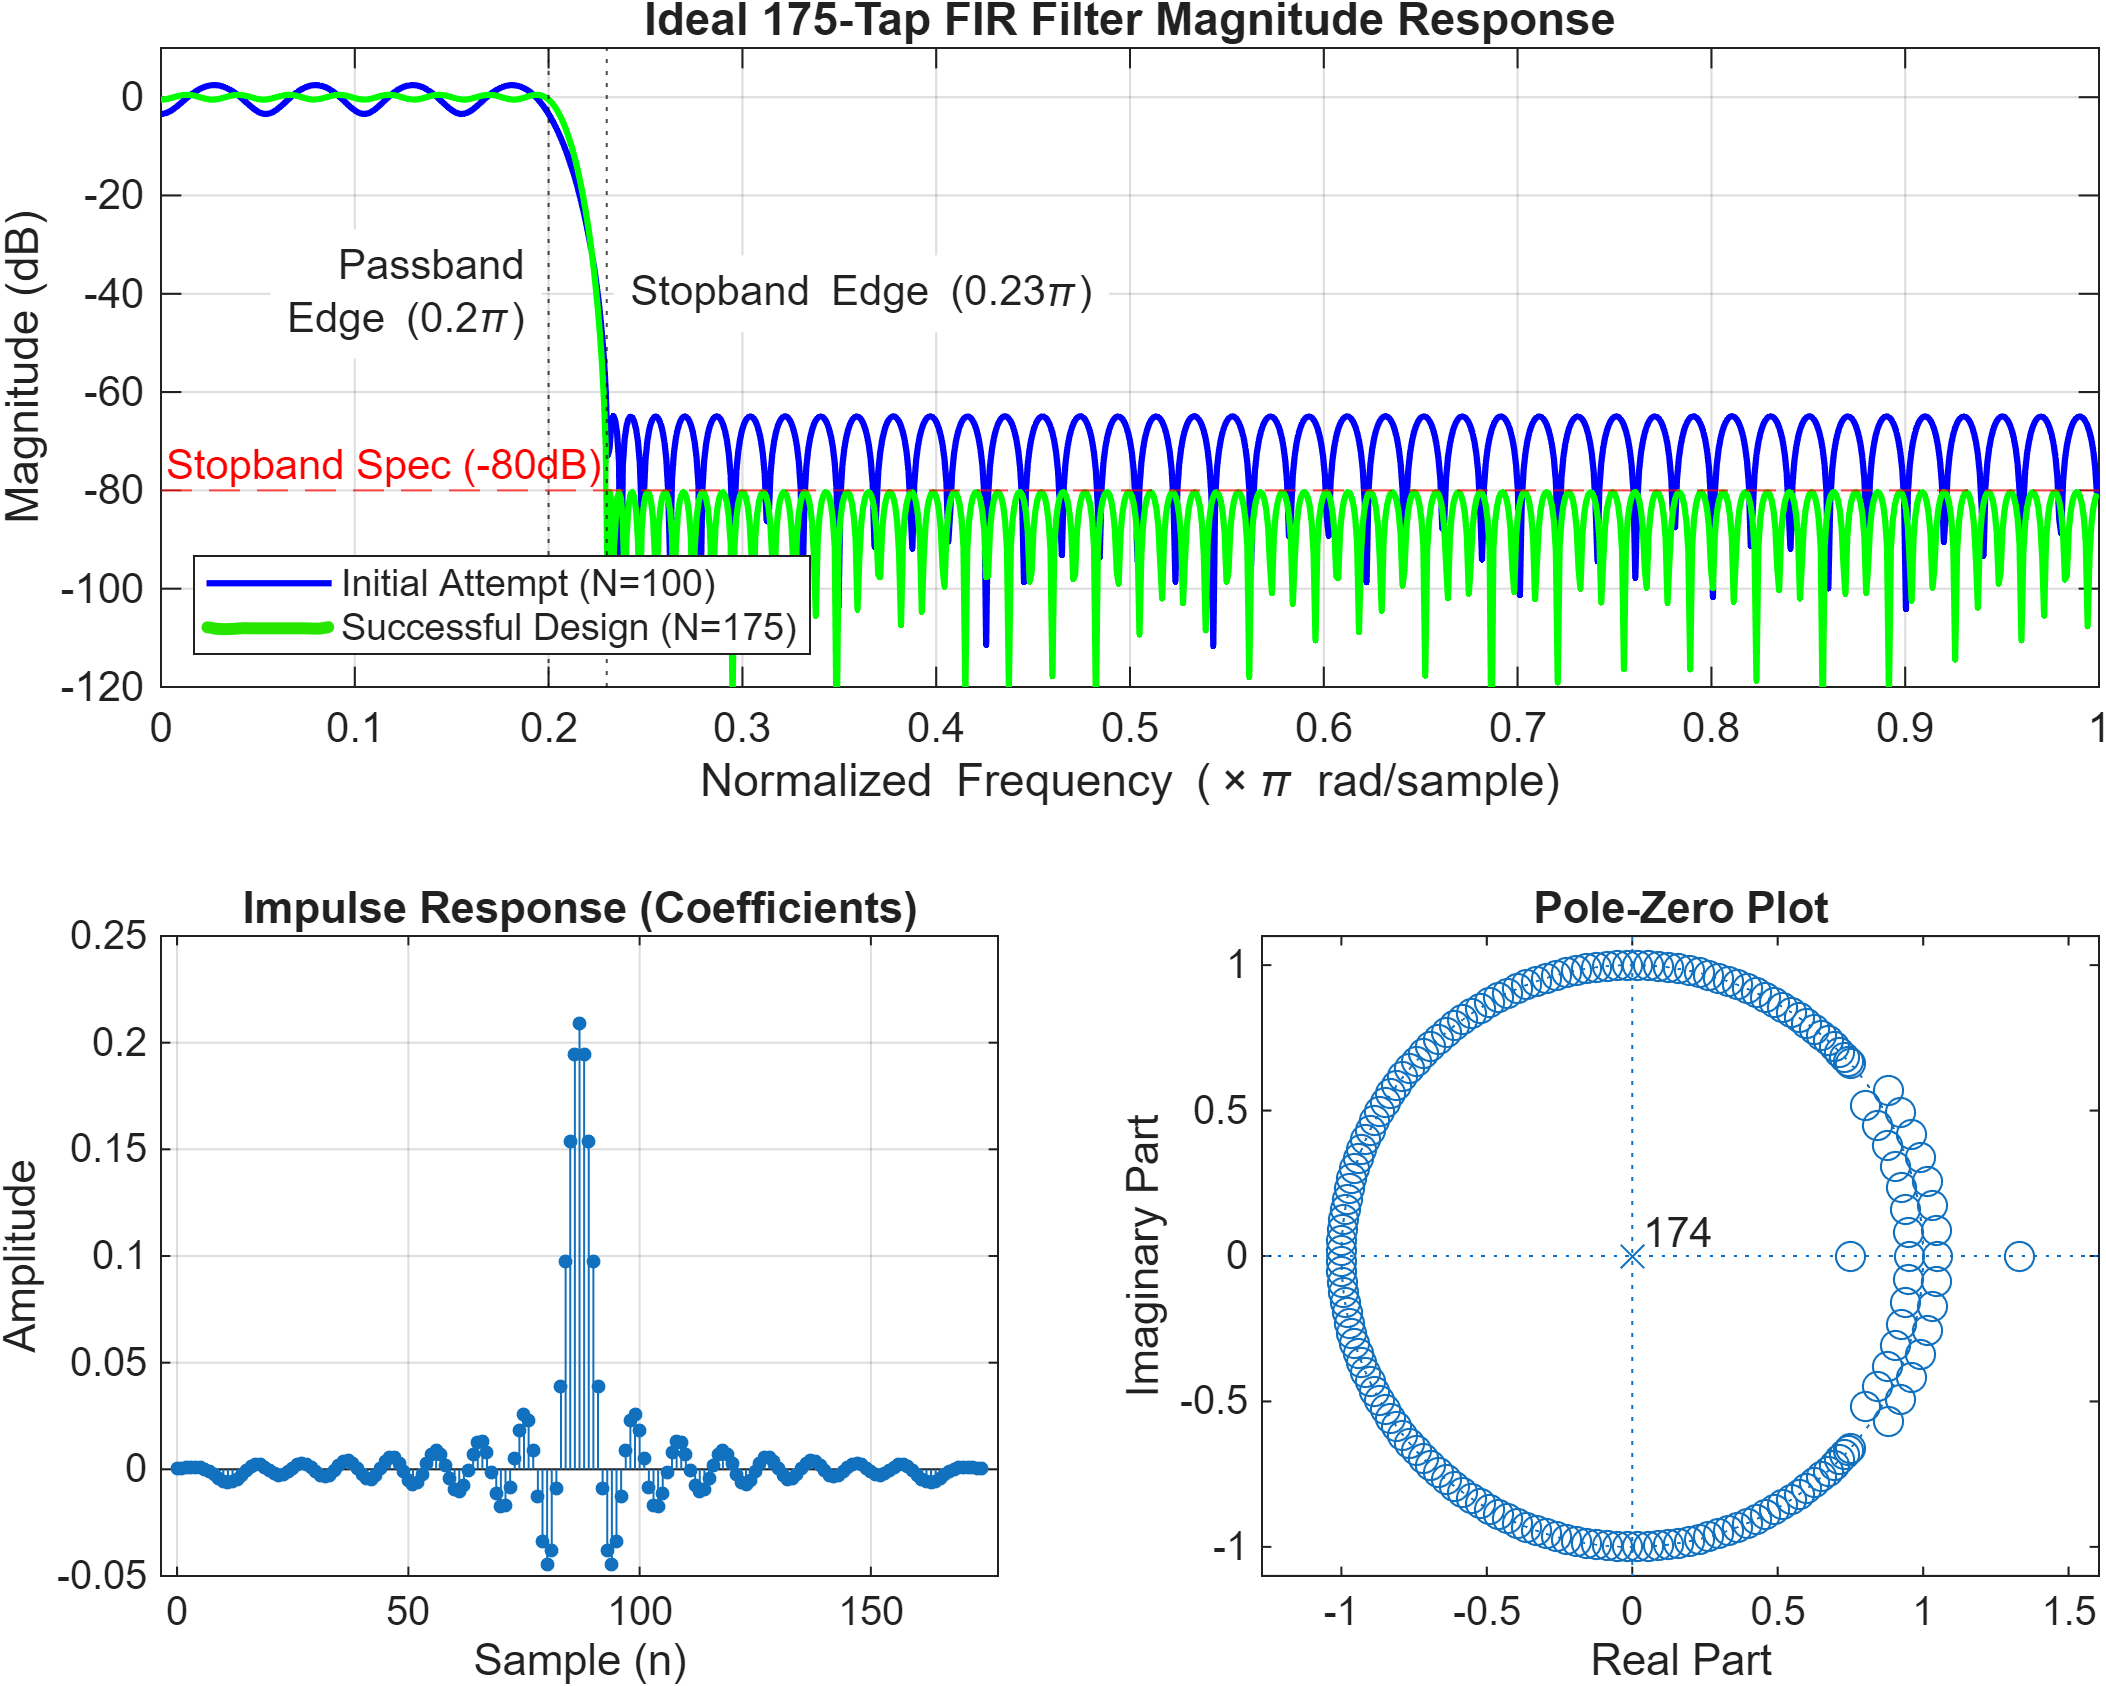
\includegraphics[width=0.95\linewidth]{images/plots/FIR_Filter_Frequency_Response.png}
    \caption{MATLAB design process: Iterated tap finding (N=175) to meet the 80 dB stopband requirement.}
\end{figure}

\subsection{Quantization and Fixed-Point Analysis}
To optimize hardware resources while maintaining signal integrity, the double-precision coefficients are quantized to a fixed-point representation. A quantization search script iterates through fractional bit widths, identifying that 23 fractional bits (Q1.22 format) are necessary to maintain the 80dB stopband spec without significant degradation.

A comprehensive datapath width analysis was performed to prevent overflow. Using the sum of absolute coefficients, the maximum possible growth of the output was calculated to determine the required number of guard bits. For the 175-tap filter with 16-bit inputs and 24-bit coefficients, a 49-bit accumulator is utilized to guarantee bit-exact correctness throughout the convolution process.


\begin{figure}[H]
    \centering
    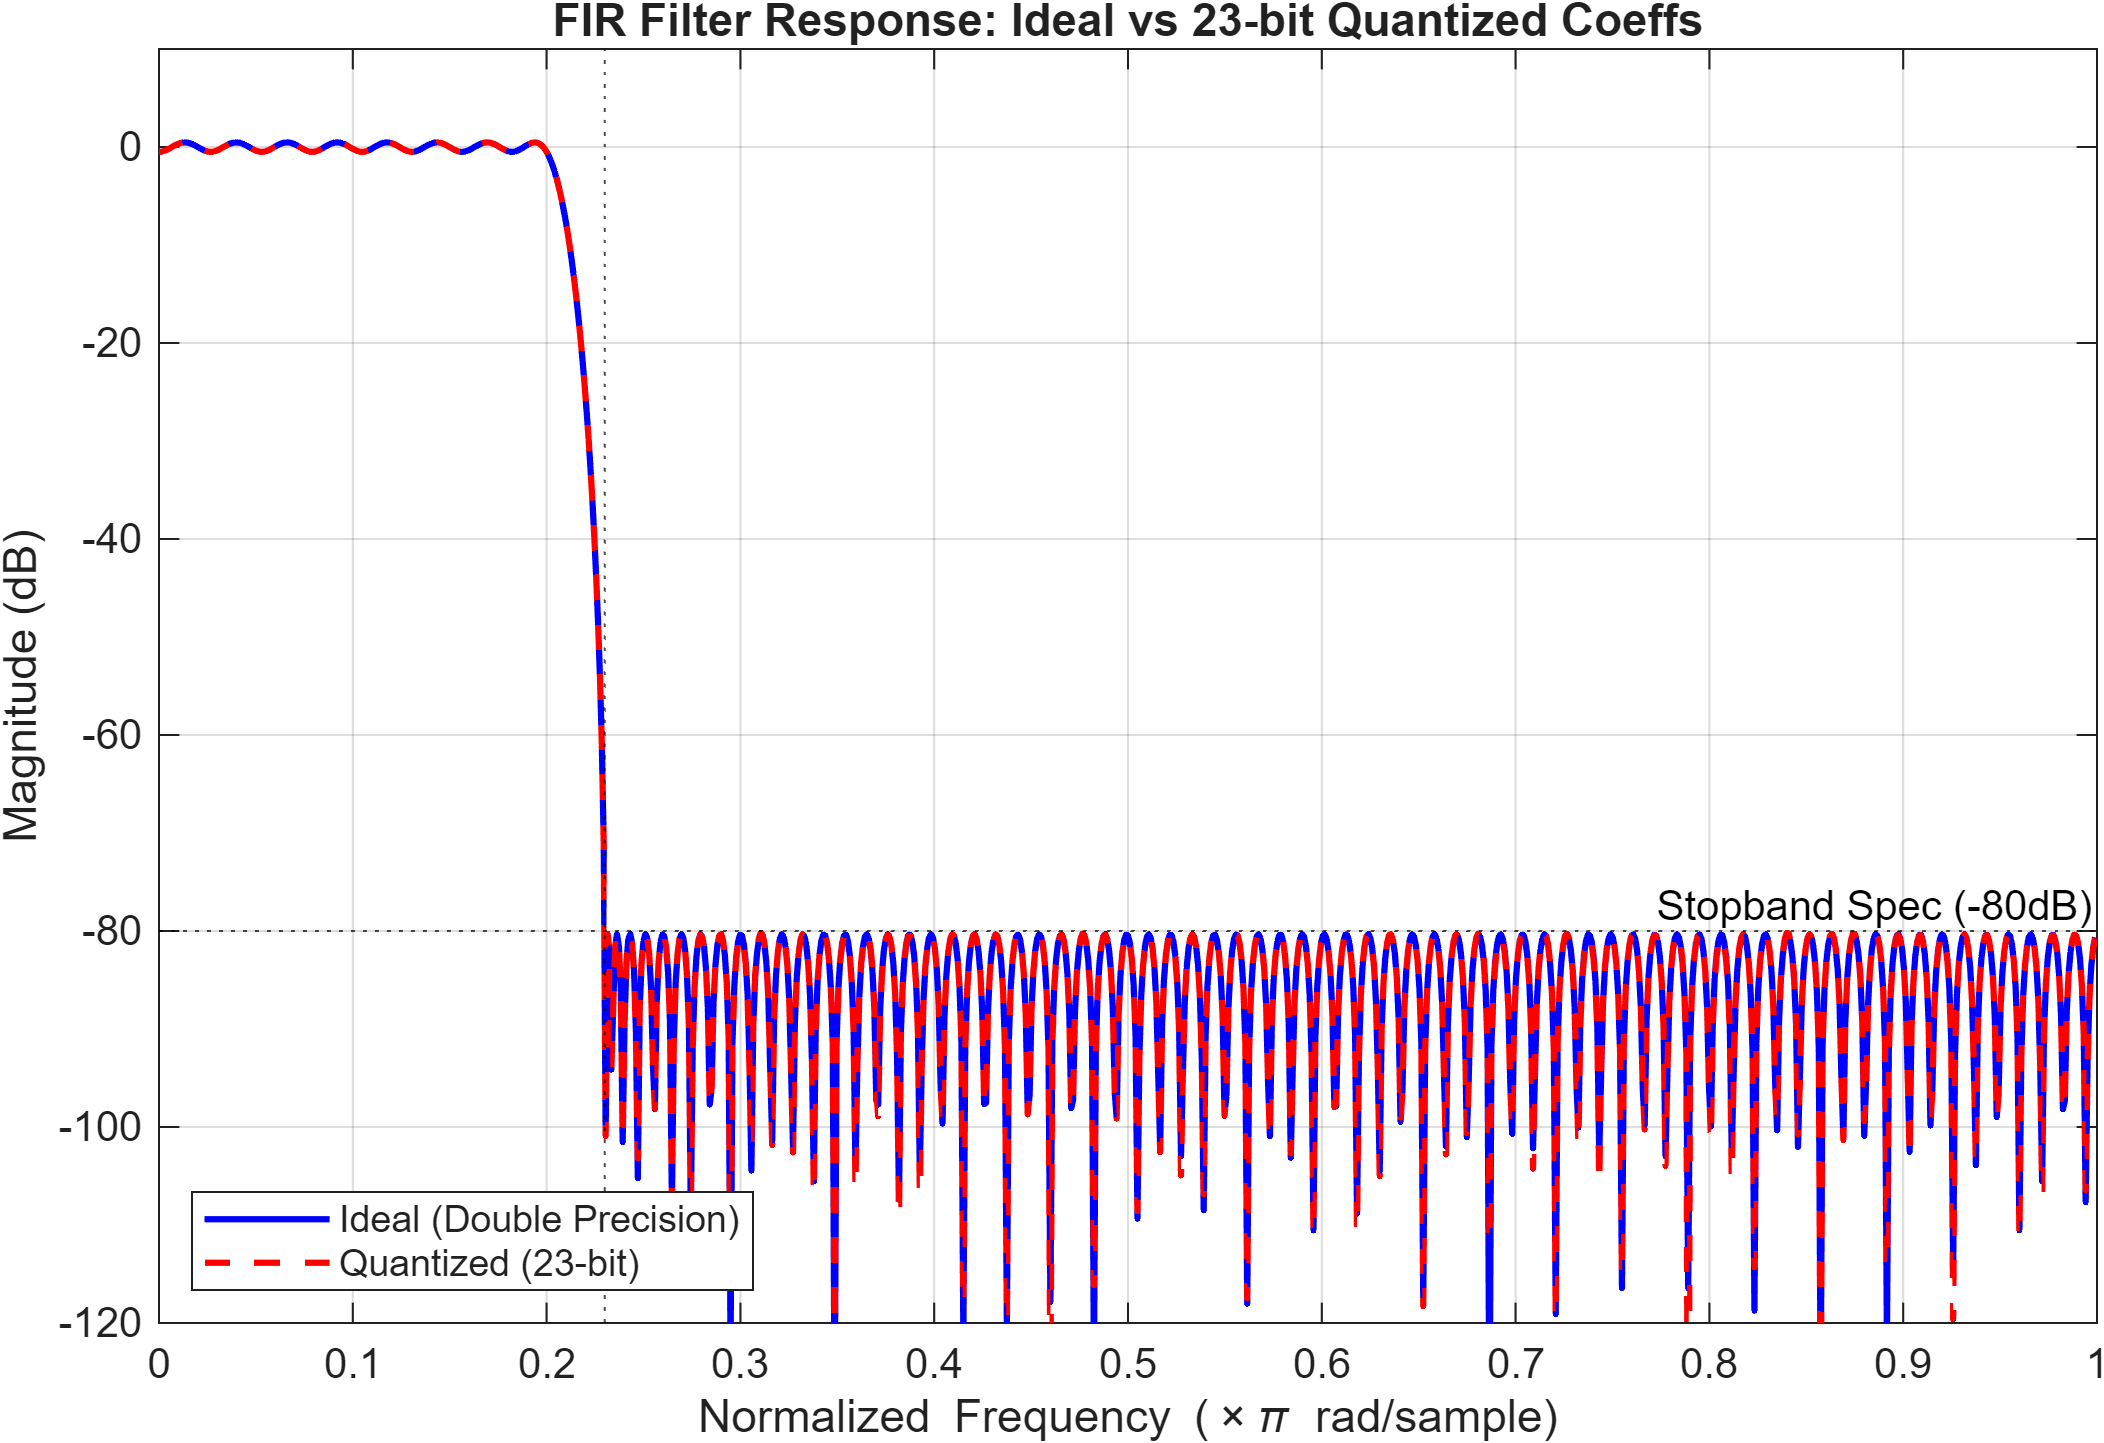
\includegraphics[width=0.95\linewidth]{images/plots/Quantization_Effects.png}
    \caption{MATLAB frequency response: Original double-precision vs. 24-bit Quantized (Q1.22) coefficients.}
\end{figure}

\subsection{Automated Hardware Integration}
An automatic design-to-hardware methodology was implemented to minimize manual error and allow for rapid design exploration. The MATLAB design environment automatically generates the following hardware artifacts:
\begin{itemize}
    \item \textbf{Coefficient Package:} A SystemVerilog package (\texttt{coeff\_pkg.sv}) containing 2's complement hexadecimal coefficients and hardware parameters (bus widths, tap count).
    \item \textbf{Verification Vectors:} Scripts generate raw binary input stimuli and bit-exact expected outputs for a wide range of test cases, including impulses, square waves, and noise.
    \item \textbf{Golden Models:} A bit-accurate MATLAB model is used to simulate the hardware's internal overflow behavior, providing a reference for RTL verification in ModelSim.
\end{itemize}

\section{Implemented Architectures}
The seven implemented architectures can be categorized into three primary architectural paradigms, progressing from baseline serial designs to high-throughput parallel and reduced-complexity structures.

\subsection{Baseline and Pipelined Designs (L=1)}
The baseline Direct Form FIR filter serves as the reference for area and power. To address the critical path bottleneck identified in synthesis, a pipelined architecture was implemented.

\begin{figure}[H]
    \centering
    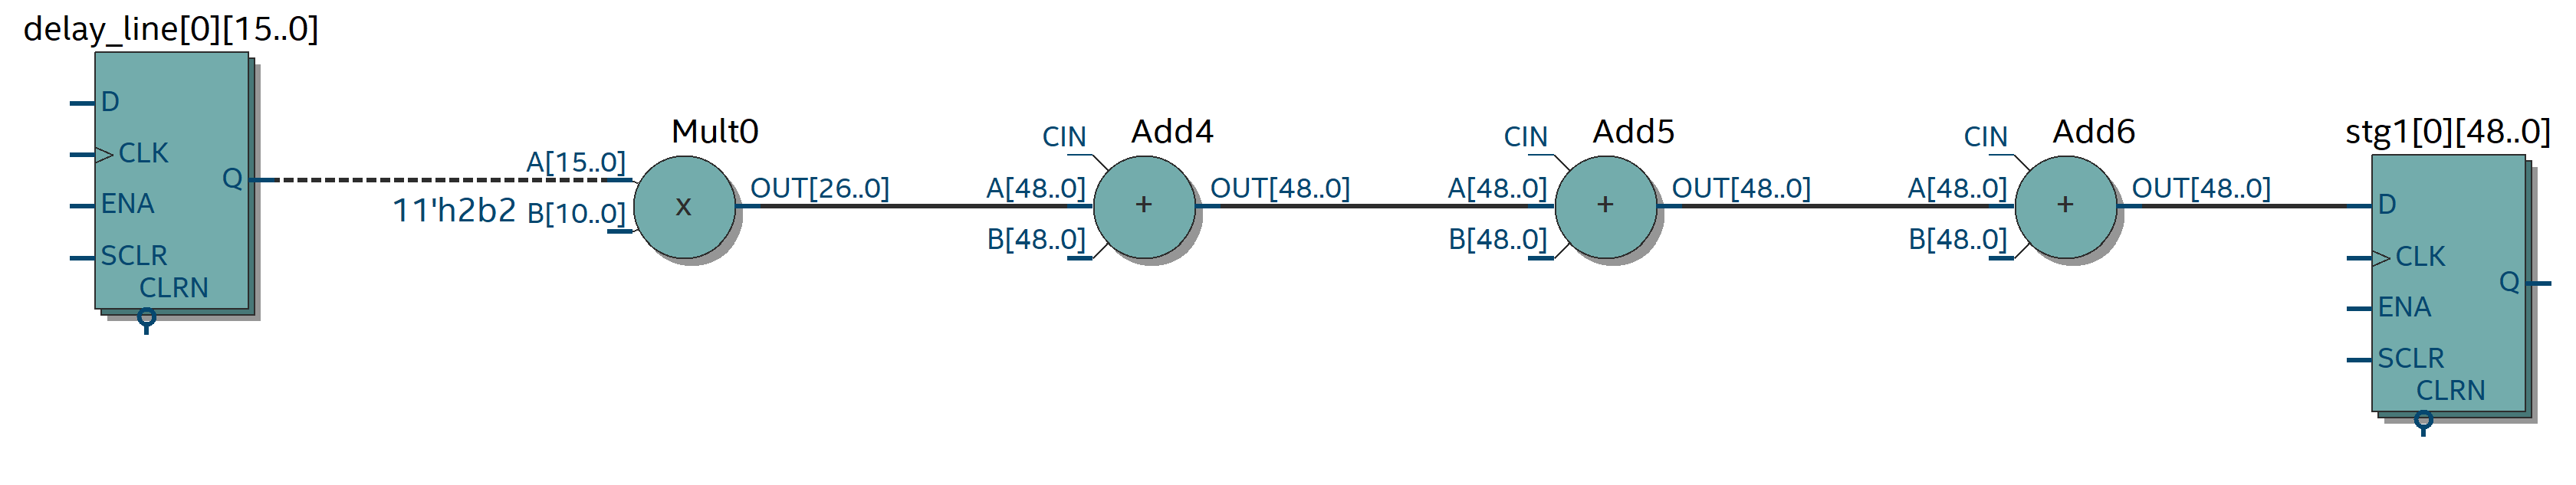
\includegraphics[width=0.95\linewidth]{images/rtl/pipelined.png}
    \caption{RTL view of a pipelined filter tap. Note the registers ($DFF$) placed after the multiplier and between adder stages to break the combinational path, enabling a significantly higher $F_{max}$.}
\end{figure}

\textbf{Implementation Details:}
\begin{itemize}
    \item \textbf{Direct Form:} Single-lane processing with a 175-tap combinational adder chain.
    \item \textbf{Pipelined FIR:} Insertion of pipeline registers to reduce the critical path to a single multiplier-adder delay. This results in a $\sim 100\%$ increase in $F_{max}$ with minimal ALM overhead.
\end{itemize}

\subsection{Parallel Polyphase Architectures (L=2, L=3)}
To increase throughput beyond the $F_{max}$ limit, parallel architectures were implemented using polyphase decomposition. This allows the filter to process $L$ samples per clock cycle.

\begin{figure}[H]
    \centering
    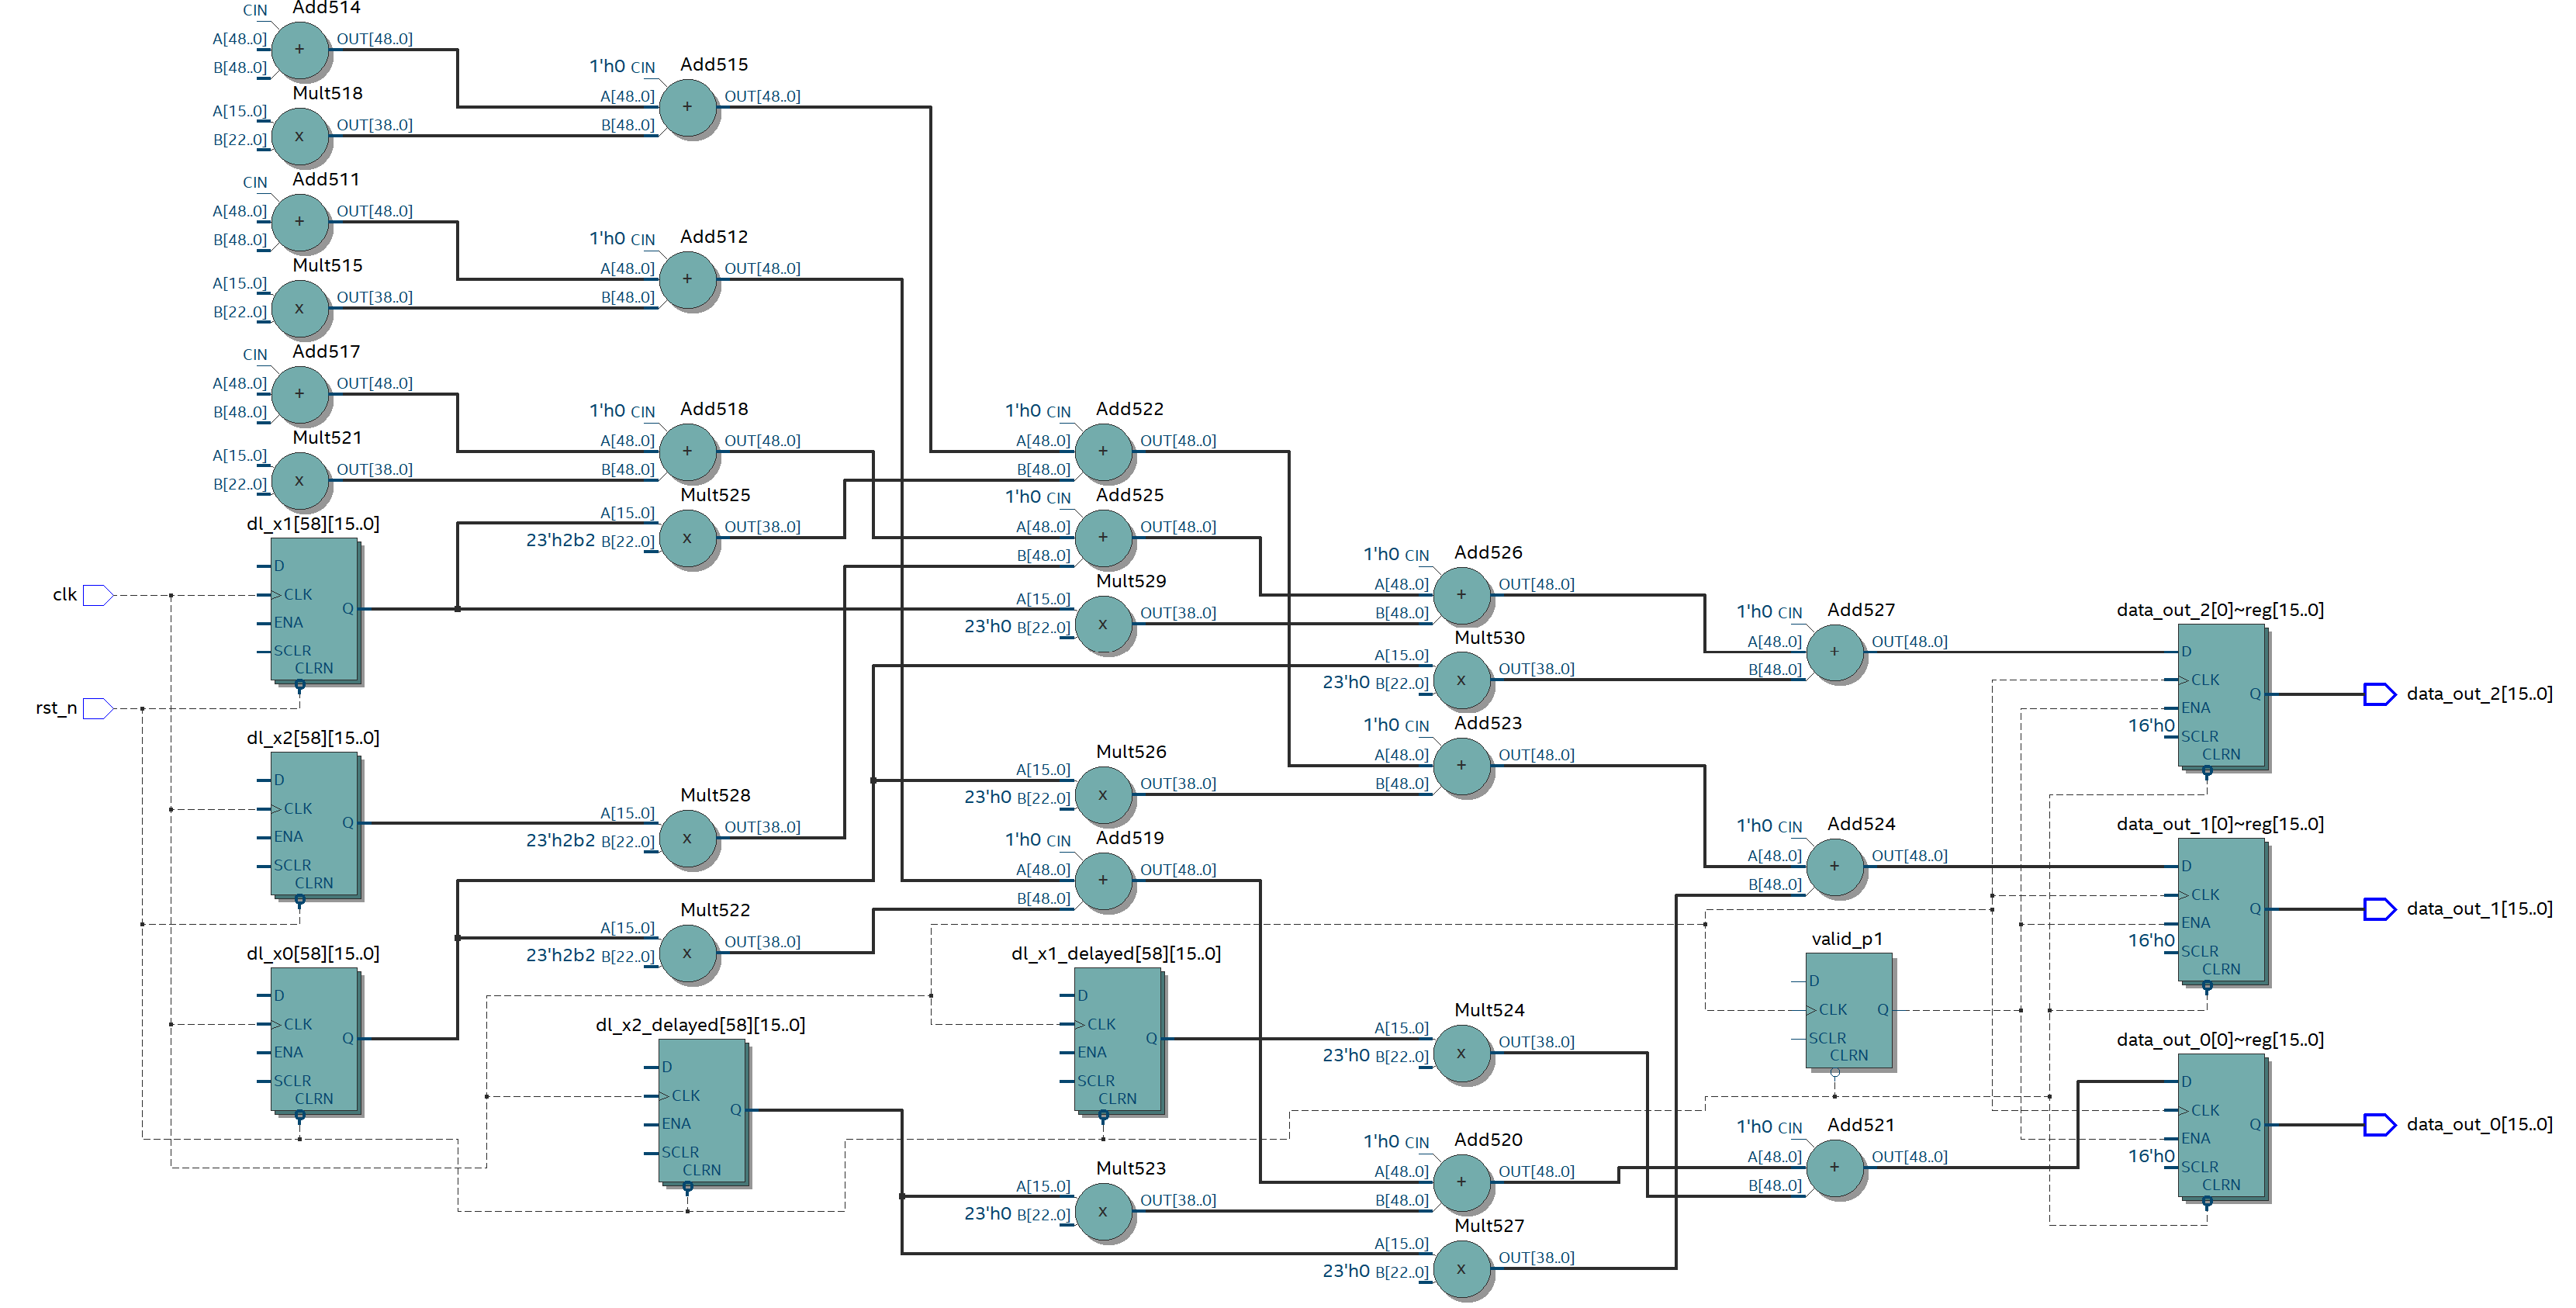
\includegraphics[width=0.95\linewidth]{images/rtl/parallel3.png}
    \caption{RTL view of the L=3 Parallel architecture. This "brute-force" polyphase decomposition utilizes 9 distinct sub-filter blocks to process three input samples ($x_0, x_1, x_2$) simultaneously.}
\end{figure}

\textbf{Architectural Analysis:}
\begin{itemize}
    \item \textbf{Throughput Scaling:} Processing $L$ samples per cycle effectively multiplies the sampling rate by $L$ while operating at a lower internal clock frequency.
    \item \textbf{Area Trade-off:} Standard parallel designs scale area linearly (or quadratically in terms of sub-filters), requiring $L^2$ sub-filter modules.
\end{itemize}

\subsection{Reduced-Complexity Parallel (Fast FIR)}
The Fast FIR Algorithm (FFA) was utilized to reduce the number of required multipliers in parallel designs. This is further optimized in the Pipelined Fast FIR L=3 design.

\begin{figure}[H]
    \centering
    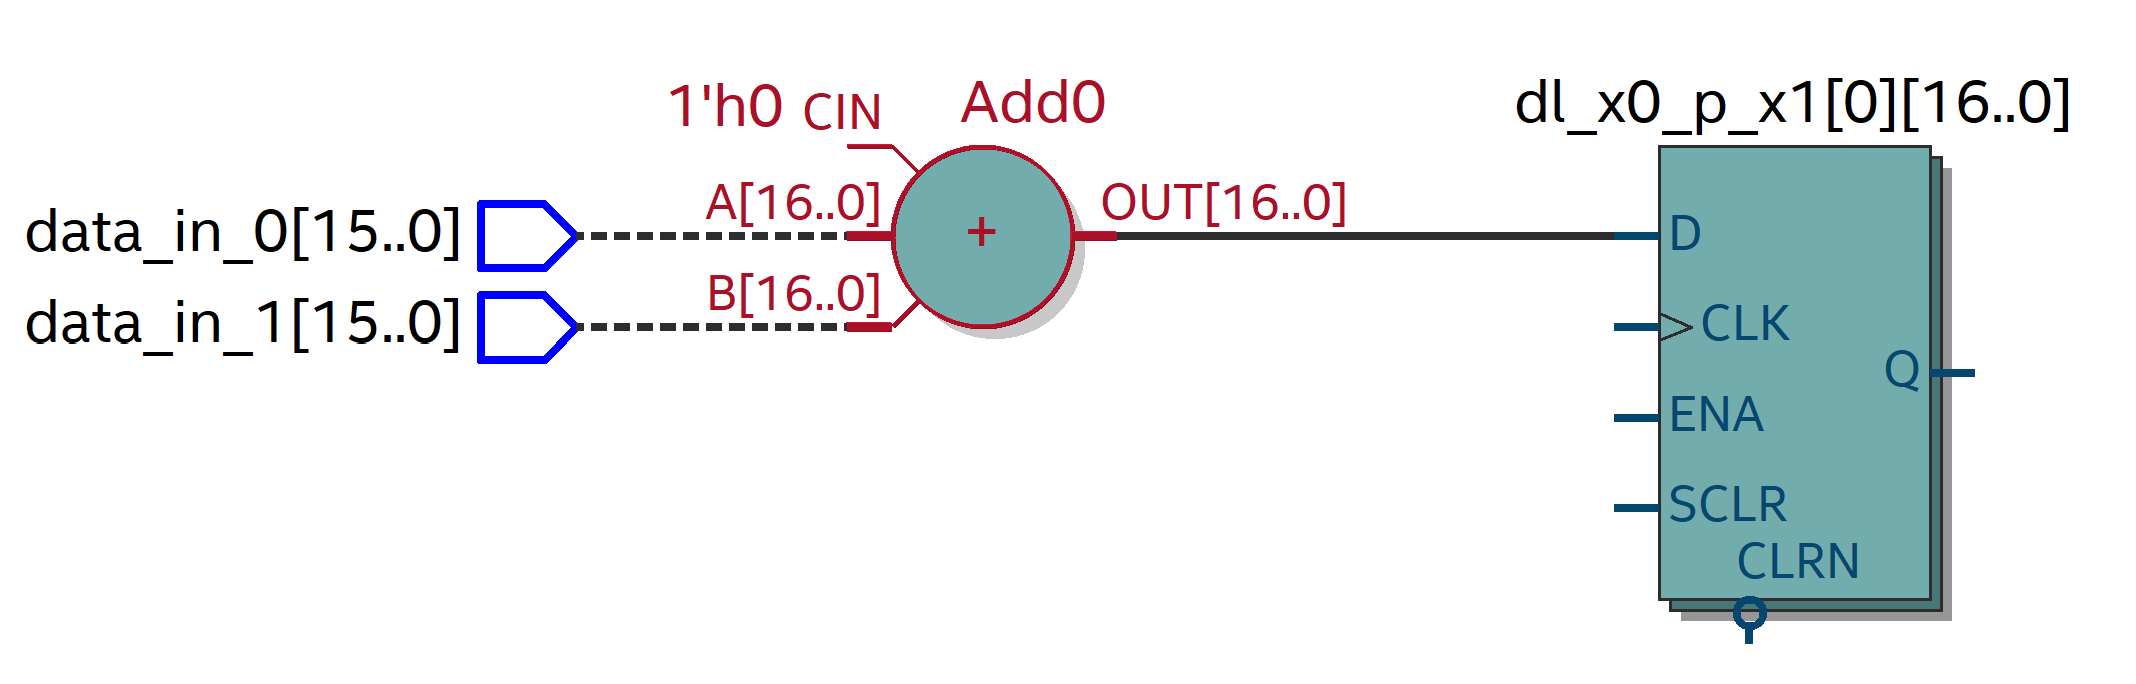
\includegraphics[width=0.95\linewidth]{images/rtl/fastpipe3.png}
    \caption{RTL view of the L=3 Fast FIR pre-processing logic. By performing pre-additions (e.g., $x_0 + x_1$) before the sub-filters, the total multiplier count is reduced from 9 to 6 for the L=3 case.}
\end{figure}

\textbf{Optimizations:}
\begin{itemize}
    \item \textbf{Multiplication Reduction:} FFA targets the most hardware-expensive operation. For $L=3$, the complexity is reduced by 33\% compared to standard parallel forms.
    \item \textbf{Hybrid Pipelining:} The optimal design (Piped FFA L=3) combines FFA logic with pipelined adder trees to achieve both low resource utilization and high frequency.
\end{itemize}


\section{Synthesis Results}
All designs were synthesized and fitted for the Intel Cyclone V FPGA (5CGXFC7C7F23C8) using Quartus Prime Lite. A notable observation is the varying DSP utilization across Parallel and Fast FIR (FFA) designs. The non-pipelined FFA L=2 and L=3 designs were synthesized using logic-based multiplier structures (0 DSPs), likely reflecting a Quartus-level resource-mapping decision for lower-speed configurations. In contrast, the high-throughput Pipelined L=3 design and baseline Parallel forms utilized 156 dedicated DSP blocks to meet more stringent timing and frequency goals.

\begin{table}[H]
\centering
\caption{Hardware Performance Comparison}
\begin{tabular}{@{}lcccc@{}}
\toprule
\textbf{Architecture} & \textbf{ALMs} & \textbf{DSP} & \textbf{$F_{max}$ (MHz)} & \textbf{Power (mW)} \\ \midrule
Direct L=1            & 2,003         & 156          & 34.1                     & 122.56              \\
Pipelined L=1         & 2,016         & 131          & 68.9                     & 93.02               \\
L=2 Parallel          & 14,119        & 156          & 36.8                     & 227.98              \\
L=3 Parallel          & 24,726        & 156          & 35.4                     & 354.13              \\
L=2 Fast FIR          & 18,785        & 0            & 35.4                     & 201.87              \\
L=3 Fast FIR          & 25,604        & 0            & 35.0                     & 302.06              \\
\textbf{Piped FFA L3} & \textbf{14,270} & \textbf{156} & \textbf{68.4}            & \textbf{137.37}     \\ \bottomrule
\end{tabular}
\end{table}

\section{Performance Analysis}
The performance of the seven implemented FIR filter architectures highlights the critical trade-offs between throughput, area utilization, and power consumption. The primary metric for comparison is the total throughput, measured in Mega-Samples Per Second (MSPS), which is defined as:
\begin{equation}
    \text{Throughput (MSPS)} = F_{max} \times L
\end{equation}
where $L$ is the number of parallel processing lanes.

\subsection{Throughput and \texorpdfstring{$F_{max}$}{Fmax} Scaling}
The baseline Direct Form architecture suffers from a long combinational critical path through the 175-tap adder chain, resulting in a modest $F_{max}$ of 34.1 MHz. By introducing pipeline registers after the multipliers and within the adder tree, the Pipelined $L=1$ design achieves a 102\% increase in frequency (68.9 MHz) with negligible ALM overhead (0.6\% increase).

Parallelism effectively scales throughput by processing $L$ samples per clock cycle. While the "brute-force" Parallel $L=3$ design achieves 106.2 MSPS, it remains limited by the low internal clock frequency of the non-pipelined sub-filters. The \textbf{Piped Fast FIR ($L=3$)} architecture \textbf{represents} the optimal design point found, achieving a peak throughput of \textbf{205.2 MSPS}. This is achieved by combining the frequency benefits of pipelining with the $L$-fold throughput multiplier of polyphase decomposition, and the algorithmic benefits of FFA.

\subsection{Area and Power Efficiency}
Logic utilization (ALM count) scales significantly with the degree of parallelism. The standard Parallel $L=3$ design requires 24,726 ALMs, a 12x increase over the serial design. The Fast FIR Algorithm (FFA) targets the reduction of hardware-expensive multipliers. Interestingly, the ALM count for the pure Fast FIR designs is higher than the standard parallel forms due to the complex pre-processing and post-reconstruction adder logic required to reduce DSP usage. However, the \textbf{Piped FFA $L=3$} architecture optimizes this logic, requiring only 14,270 ALMs to achieve its high throughput.

Power efficiency, measured as power per MSPS, is highest in the Piped FFA $L=3$ design. It consumes 137.37 mW to deliver 205.2 MSPS ($\sim 0.67$ mW/MSPS), compared to the Direct Form's 3.59 mW/MSPS. This demonstrates that hybrid architectures combining algorithmic reduction (Fast FIR) and structural optimization (pipelining) provide the most efficient utilization of FPGA resources for high-speed DSP tasks.



\section{Conclusion}
The hardware simulation and performance analysis demonstrates a clear trade-off between throughput, area utilization, and power consumption. The Piped FFA $L=3$ architecture represents the optimal design point found, achieving a peak throughput of 205.2 MSPS with minimal resource utilization. These results are supported by the ground truth MATLAB simulations, which show bit-exact matches with the RTL outputs across all stimuli, as well as the advanced architecture waveforms matching the baseline, Direct Form, architecture. Further scalability can be explored by extending these architectures to higher parallelization factors ($L>3$) or integrating adaptive filtering capabilities within the established high-throughput framework.

\newpage
\section{Functional Verification}
RTL verification shows bit-exact matches with MATLAB models across all stimuli. The following waveforms demonstrate functional correctness for each of the seven architectures.

\subsection{Full Signal Test}
\subsubsection{Direct Form}
Check for the bit-exact match and total simulation time alignment between the RTL and MATLAB outputs.
\begin{figure}[H]
    \centering
    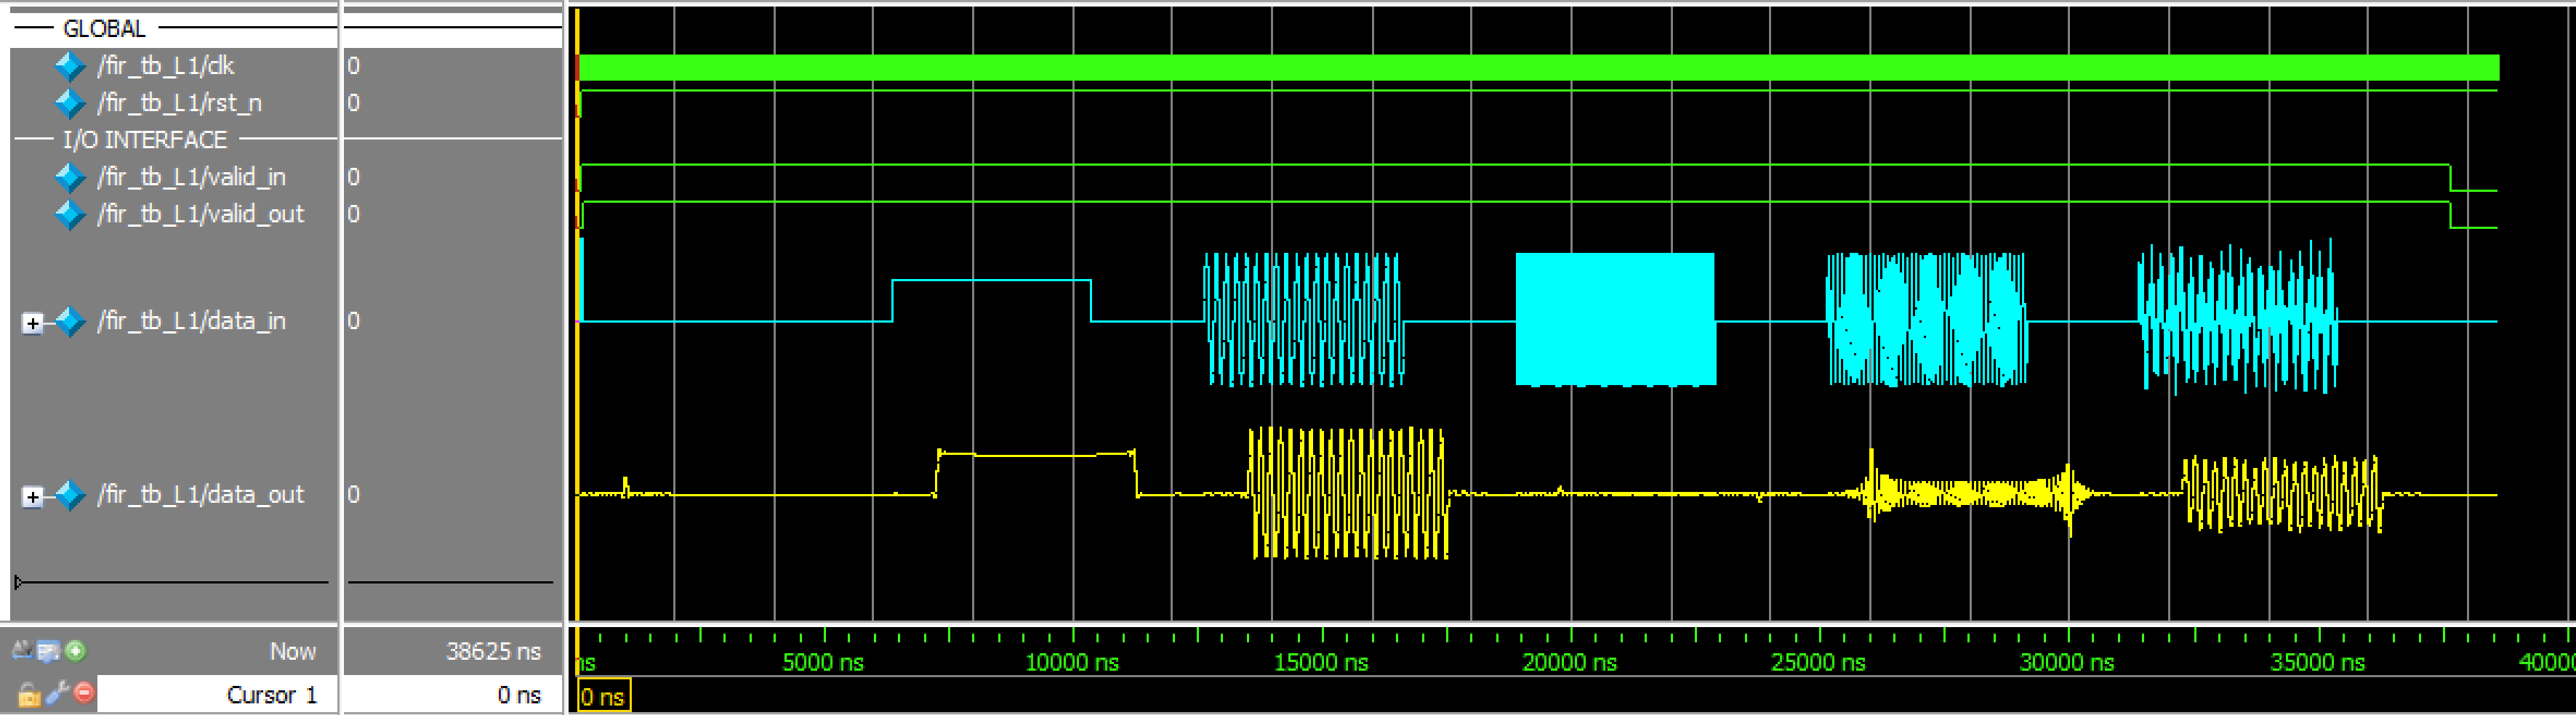
\includegraphics[width=0.95\linewidth]{images/waveforms/direct/full.png}
    \caption{Full Signal Test: Direct Form.}
\end{figure}

\subsubsection{Pipelined FIR}
Observe the match while considering the fixed pipeline delay introduced by the added registers.
\begin{figure}[H]
    \centering
    
\includegraphics[width=0.95\linewidth]{images/waveforms/pipelined/full.png}
    \caption{Full Signal Test: Pipelined FIR.}
\end{figure}

\subsubsection{Parallel L=2}
Note the multiple signals ($y_0, y_1$) processing the interleaved data streams.
\begin{figure}[H]
    \centering
    
\includegraphics[width=0.95\linewidth]{images/waveforms/parallel2/full.png}
    \caption{Full Signal Test: Parallel L=2 (Lanes).}
\end{figure}
Confirm the reconstructed output matches the direct serial form for the L=2 case.
\begin{figure}[H]
    \centering
    
\includegraphics[width=0.95\linewidth]{images/waveforms/parallel2/reconstruction.png}
    \caption{Full Signal Test: Parallel L=2 (Reconstructed).}
\end{figure}

\subsubsection{Fast FIR L=2}
Observe the sub-filter outputs ($y_0, y_1$) implementing the Fast FIR algorithm logic.
\begin{figure}[H]
    \centering
    
\includegraphics[width=0.95\linewidth]{images/waveforms/fast2/full.png}
    \caption{Full Signal Test: Fast FIR L=2 (Lanes).}
\end{figure}
Verify the bit-exact match of the reconstructed $L=2$ Fast FIR output.
\begin{figure}[H]
    \centering
    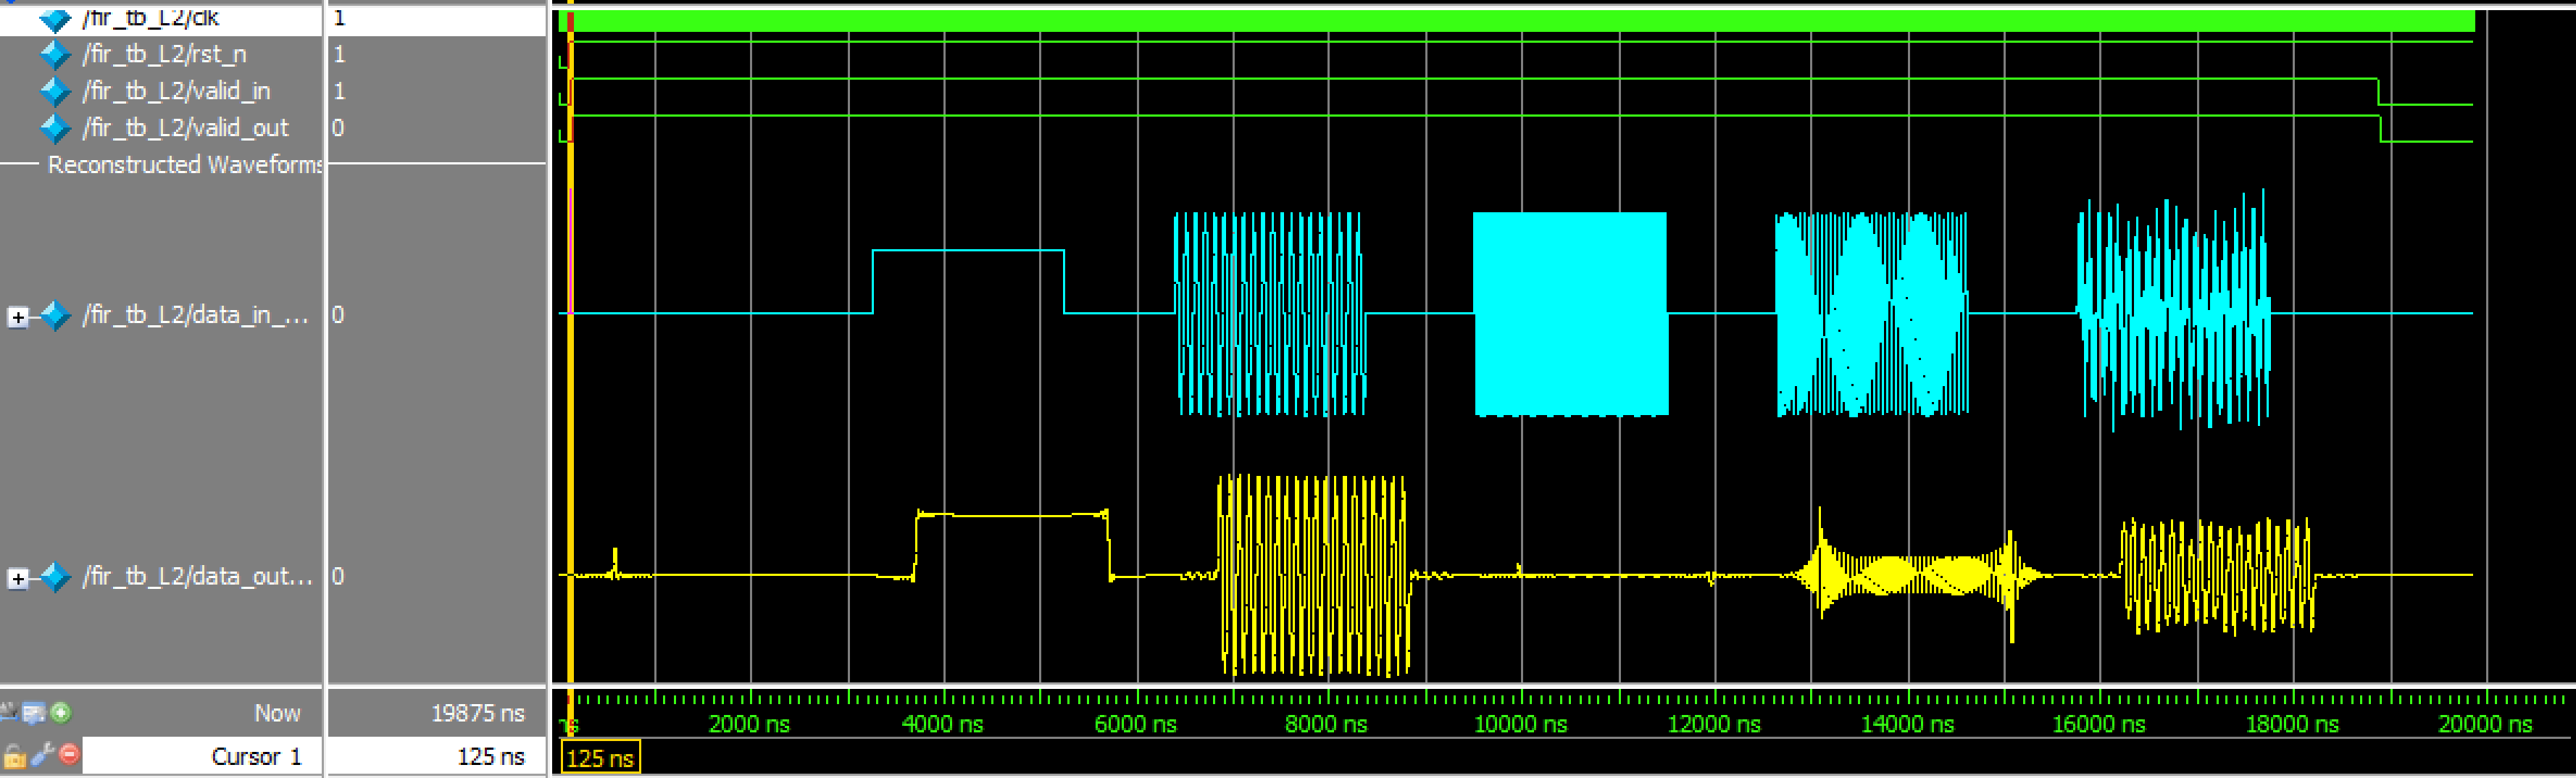
\includegraphics[width=0.95\linewidth]{images/waveforms/fast2/reconstruction.png}
    \caption{Full Signal Test: Fast FIR L=2 (Reconstructed).}
\end{figure}

\subsubsection{Parallel L=3}
Note the three parallel lanes ($y_0, y_1, y_2$) operating at $1/3$ the sampling rate.
\begin{figure}[H]
    \centering
    
\includegraphics[width=0.95\linewidth]{images/waveforms/parallel3/full.png}
    \caption{Full Signal Test: Parallel L=3 (Lanes).}
\end{figure}
Confirm the reconstructed output matches the $L=3$ serial reference.
\begin{figure}[H]
    \centering
    
\includegraphics[width=0.95\linewidth]{images/waveforms/parallel3/reconstructed.png}
    \caption{Full Signal Test: Parallel L=3 (Reconstructed).}
\end{figure}

\subsubsection{Fast FIR L=3}
Observe the multiple sub-filter outputs that form the $L=3$ parallel response.
\begin{figure}[H]
    \centering
    
\includegraphics[width=0.95\linewidth]{images/waveforms/fast3/full.png}
    \caption{Full Signal Test: Fast FIR L=3 (Lanes).}
\end{figure}
Verify the bit-exact reconstruction of the $L=3$ Fast FIR architecture.
\begin{figure}[H]
    \centering
    
\includegraphics[width=0.95\linewidth]{images/waveforms/fast3/reconstruction.png}
    \caption{Full Signal Test: Fast FIR L=3 (Reconstructed).}
\end{figure}

\subsubsection{Pipelined Fast FIR L=3}
Note the high-performance pipelined lanes delivering processed throughput at three samples per cycle.
\begin{figure}[H]
    \centering
    
\includegraphics[width=0.95\linewidth]{images/waveforms/fastpipe3/full.png}
    \caption{Full Signal Test: Pipelined Fast FIR L=3 (Lanes).}
\end{figure}
Confirm the final reconstructed output for the Pipelined Fast FIR L=3 matches the reference.
\begin{figure}[H]
    \centering
    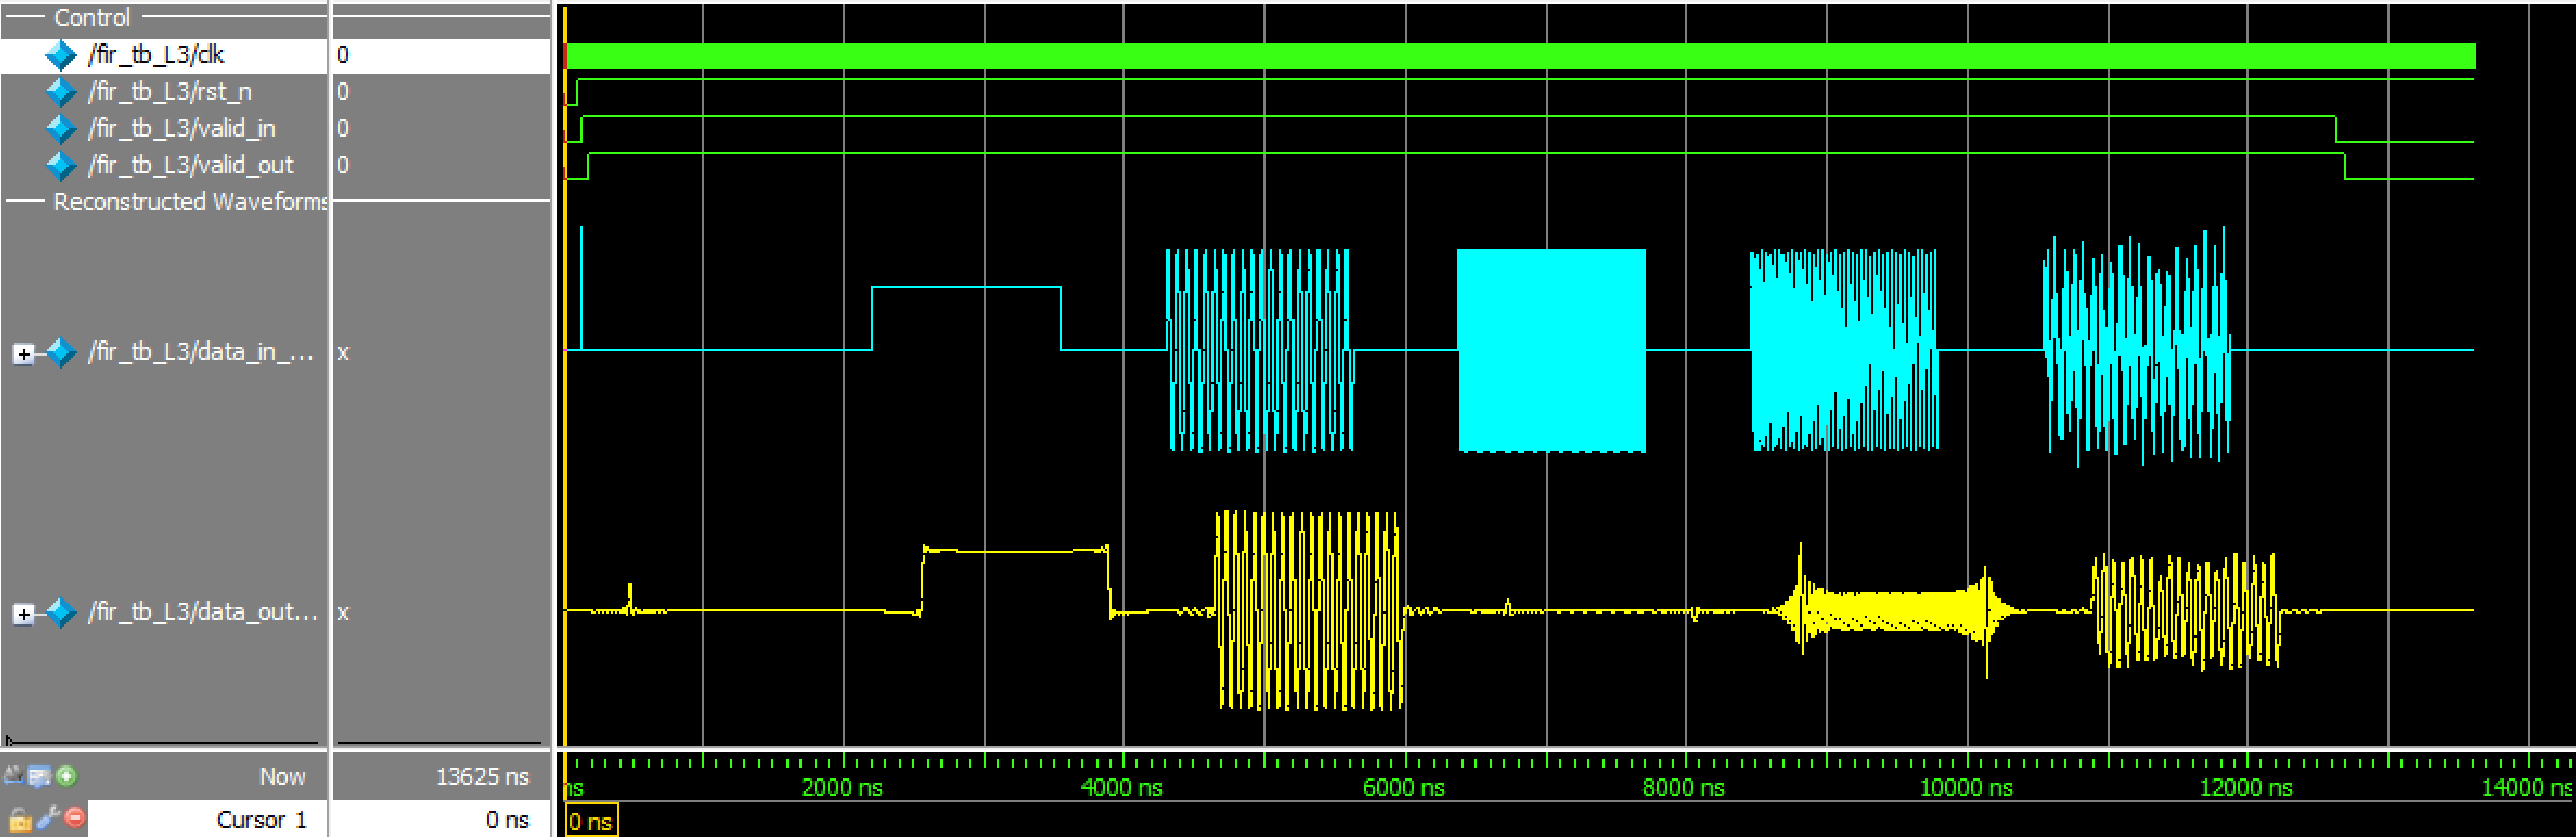
\includegraphics[width=0.95\linewidth]{images/waveforms/fastpipe3/reconstructed.png}
    \caption{Full Signal Test: Pipelined Fast FIR L=3 (Reconstructed).}
\end{figure}

\subsection{Impulse Response}
\subsubsection{Direct Form}
Check for the 175 symmetric filter coefficients and the characteristic peak at the center tap.
\begin{figure}[H]
    \centering
    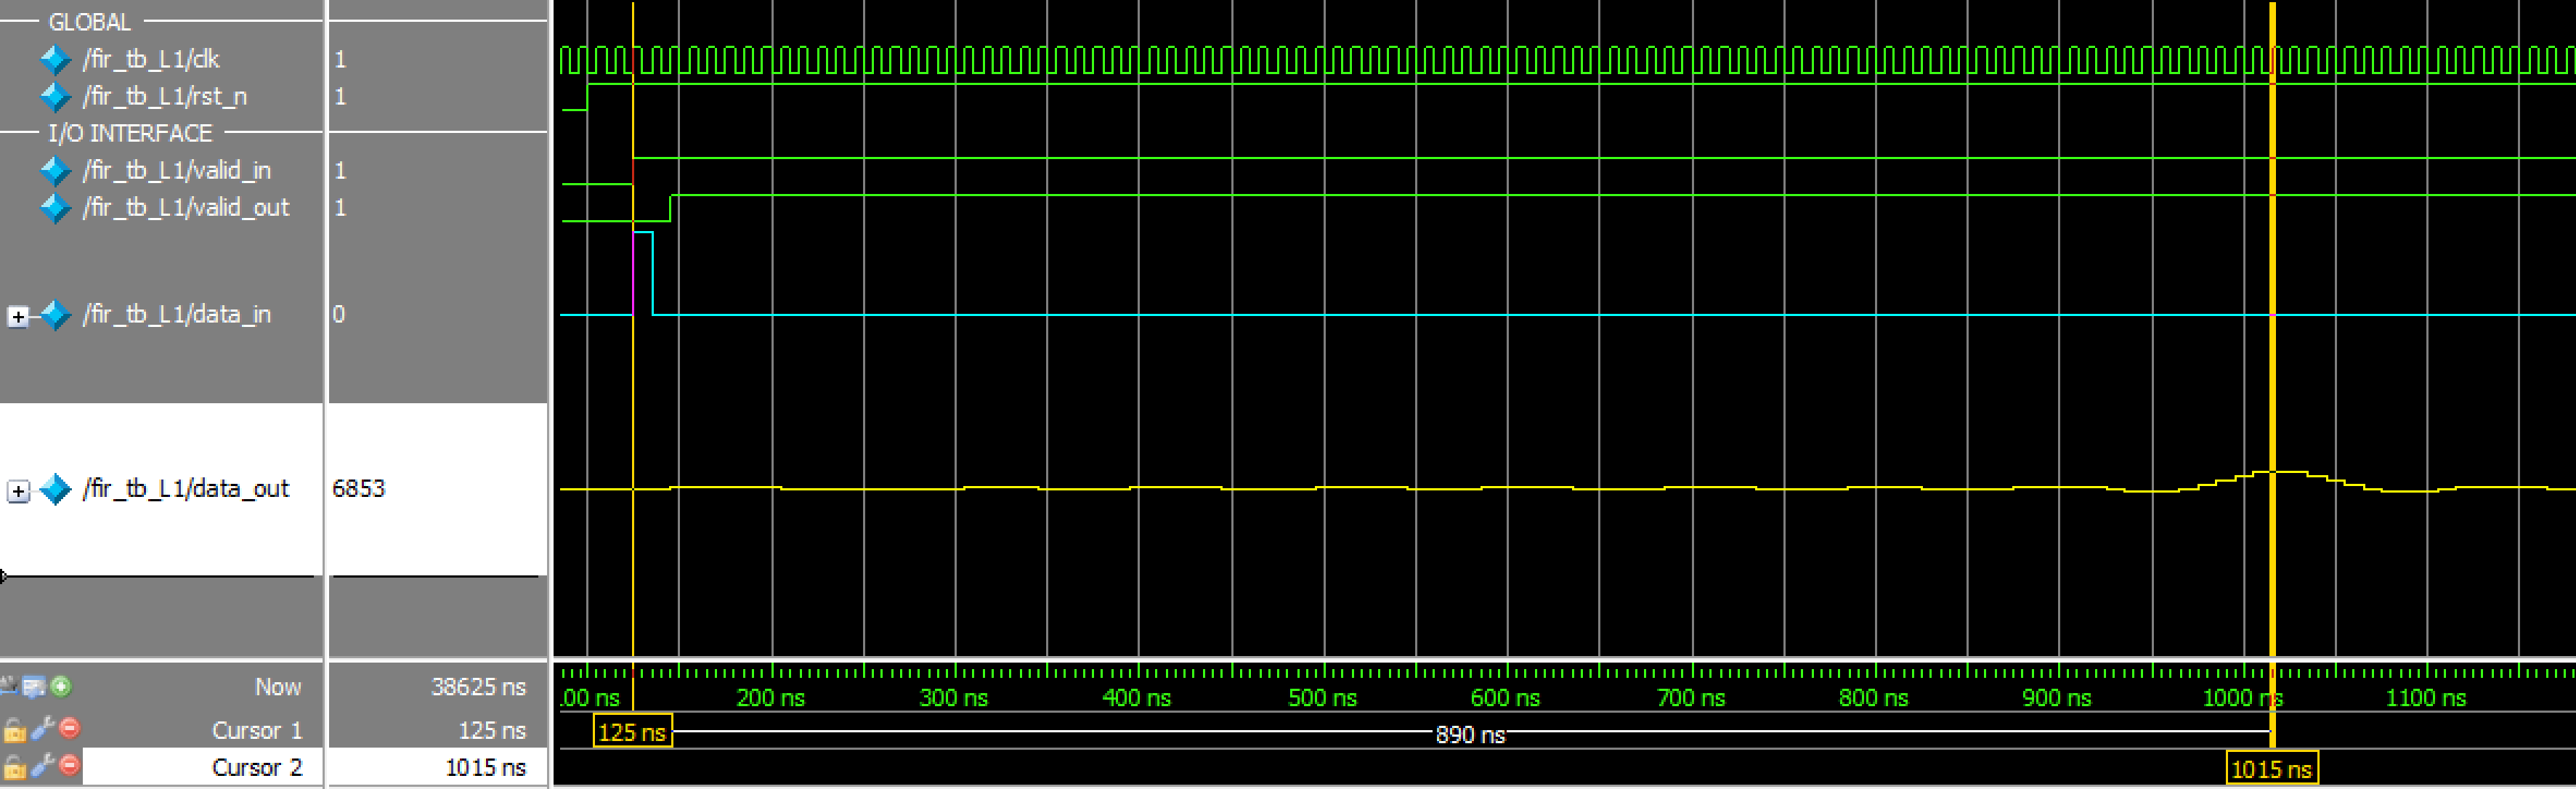
\includegraphics[width=0.95\linewidth]{images/waveforms/direct/impulse.png}
    \caption{Impulse Response: Direct Form.}
\end{figure}
\subsubsection{Pipelined FIR}
Verify the impulse response matches the coefficients, noting the fixed delay from pipelining.
\begin{figure}[H]
    \centering
    
\includegraphics[width=0.95\linewidth]{images/waveforms/pipelined/impulse.png}
    \caption{Impulse Response: Pipelined FIR.}
\end{figure}
\subsubsection{Parallel L=2}
Observe how the impulse response is distributed across the parallel processing lanes.
\begin{figure}[H]
    \centering
    
\includegraphics[width=0.95\linewidth]{images/waveforms/parallel2/impulse.png}
    \caption{Impulse Response: Parallel L=2.}
\end{figure}
\subsubsection{Fast FIR L=2}
Verify the Fast FIR logic correctly reproduces the impulse response through its sub-filter structures.
\begin{figure}[H]
    \centering
    
\includegraphics[width=0.95\linewidth]{images/waveforms/fast2/impulse.png}
    \caption{Impulse Response: Fast FIR L=2.}
\end{figure}
\subsubsection{Parallel L=3}
Note the interleaving of the impulse response across the three parallel output signals.
\begin{figure}[H]
    \centering
    
\includegraphics[width=0.95\linewidth]{images/waveforms/parallel3/impulse.png}
    \caption{Impulse Response: Parallel L=3.}
\end{figure}
\subsubsection{Fast FIR L=3}
Confirm that the reduced-complexity sub-filters correctly reconstruct the 175-tap impulse response.
\begin{figure}[H]
    \centering
    
\includegraphics[width=0.95\linewidth]{images/waveforms/fast3/impulse.png}
    \caption{Impulse Response: Fast FIR L=3.}
\end{figure}
\subsubsection{Pipelined Fast FIR L=3}
Observe the high-throughput impulse response reconstruction for the optimized pipelined architecture.
\begin{figure}[H]
    \centering
    
\includegraphics[width=0.95\linewidth]{images/waveforms/fastpipe3/impulse.png}
    \caption{Impulse Response: Pipelined Fast FIR L=3.}
\end{figure}

\subsection{Square Wave}
\subsubsection{Direct Form}
Identify the Gibbs phenomenon and symmetrical ringing at the transitions of the square wave.
\begin{figure}[H]
    \centering
    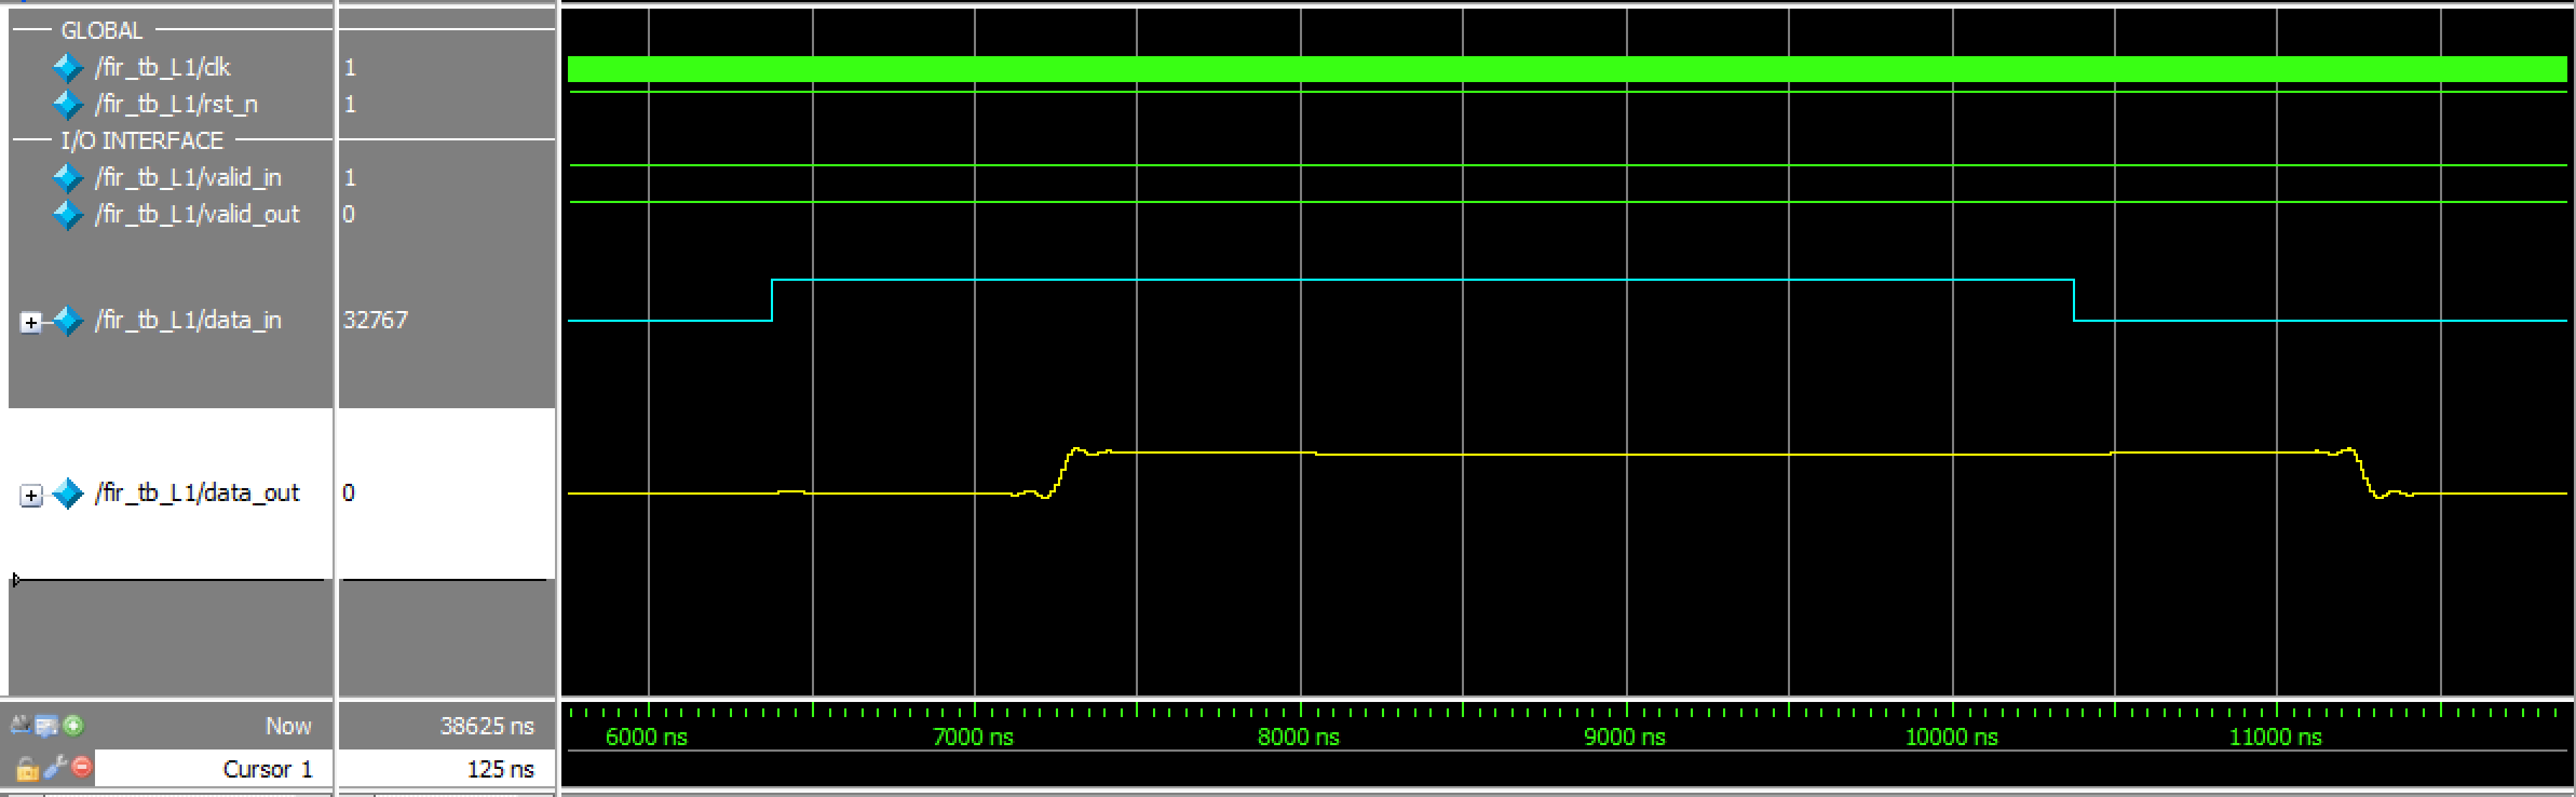
\includegraphics[width=0.95\linewidth]{images/waveforms/direct/square.png}
    \caption{Square Wave: Direct Form.}
\end{figure}
\subsubsection{Pipelined FIR}
Observe the transient response while accounting for the cycles of internal register delay.
\begin{figure}[H]
    \centering
    
\includegraphics[width=0.95\linewidth]{images/waveforms/pipelined/square.png}
    \caption{Square Wave: Pipelined FIR.}
\end{figure}
\subsubsection{Parallel L=2}
Note how the sharp transitions are handled across the parallel lanes in the polyphase structure.
\begin{figure}[H]
    \centering
    
\includegraphics[width=0.95\linewidth]{images/waveforms/parallel2/square.png}
    \caption{Square Wave: Parallel L=2.}
\end{figure}
\subsubsection{Fast FIR L=2}
Verify the step response symmetry for the Fast FIR implementation.
\begin{figure}[H]
    \centering
    
\includegraphics[width=0.95\linewidth]{images/waveforms/fast2/square.png}
    \caption{Square Wave: Fast FIR L=2.}
\end{figure}
\subsubsection{Parallel L=3}
Observe the transient response across the three parallel output lanes.
\begin{figure}[H]
    \centering
    
\includegraphics[width=0.95\linewidth]{images/waveforms/parallel3/square.png}
    \caption{Square Wave: Parallel L=3.}
\end{figure}
\subsubsection{Fast FIR L=3}
Confirm that the square wave stimulus is correctly filtered by the $L=3$ Fast FIR sub-filters.
\begin{figure}[H]
    \centering
    
\includegraphics[width=0.95\linewidth]{images/waveforms/fast3/square.png}
    \caption{Square Wave: Fast FIR L=3.}
\end{figure}
\subsubsection{Pipelined Fast FIR L=3}
Verify the high-throughput transient response for the most complex architecture.
\begin{figure}[H]
    \centering
    
\includegraphics[width=0.95\linewidth]{images/waveforms/fastpipe3/square.png}
    \caption{Square Wave: Pipelined Fast FIR L=3.}
\end{figure}

\subsection{Low Frequency}
\subsubsection{Direct Form}
Verify that the low-frequency passband signal is transmitted with minimal attenuation.
\begin{figure}[H]
    \centering
    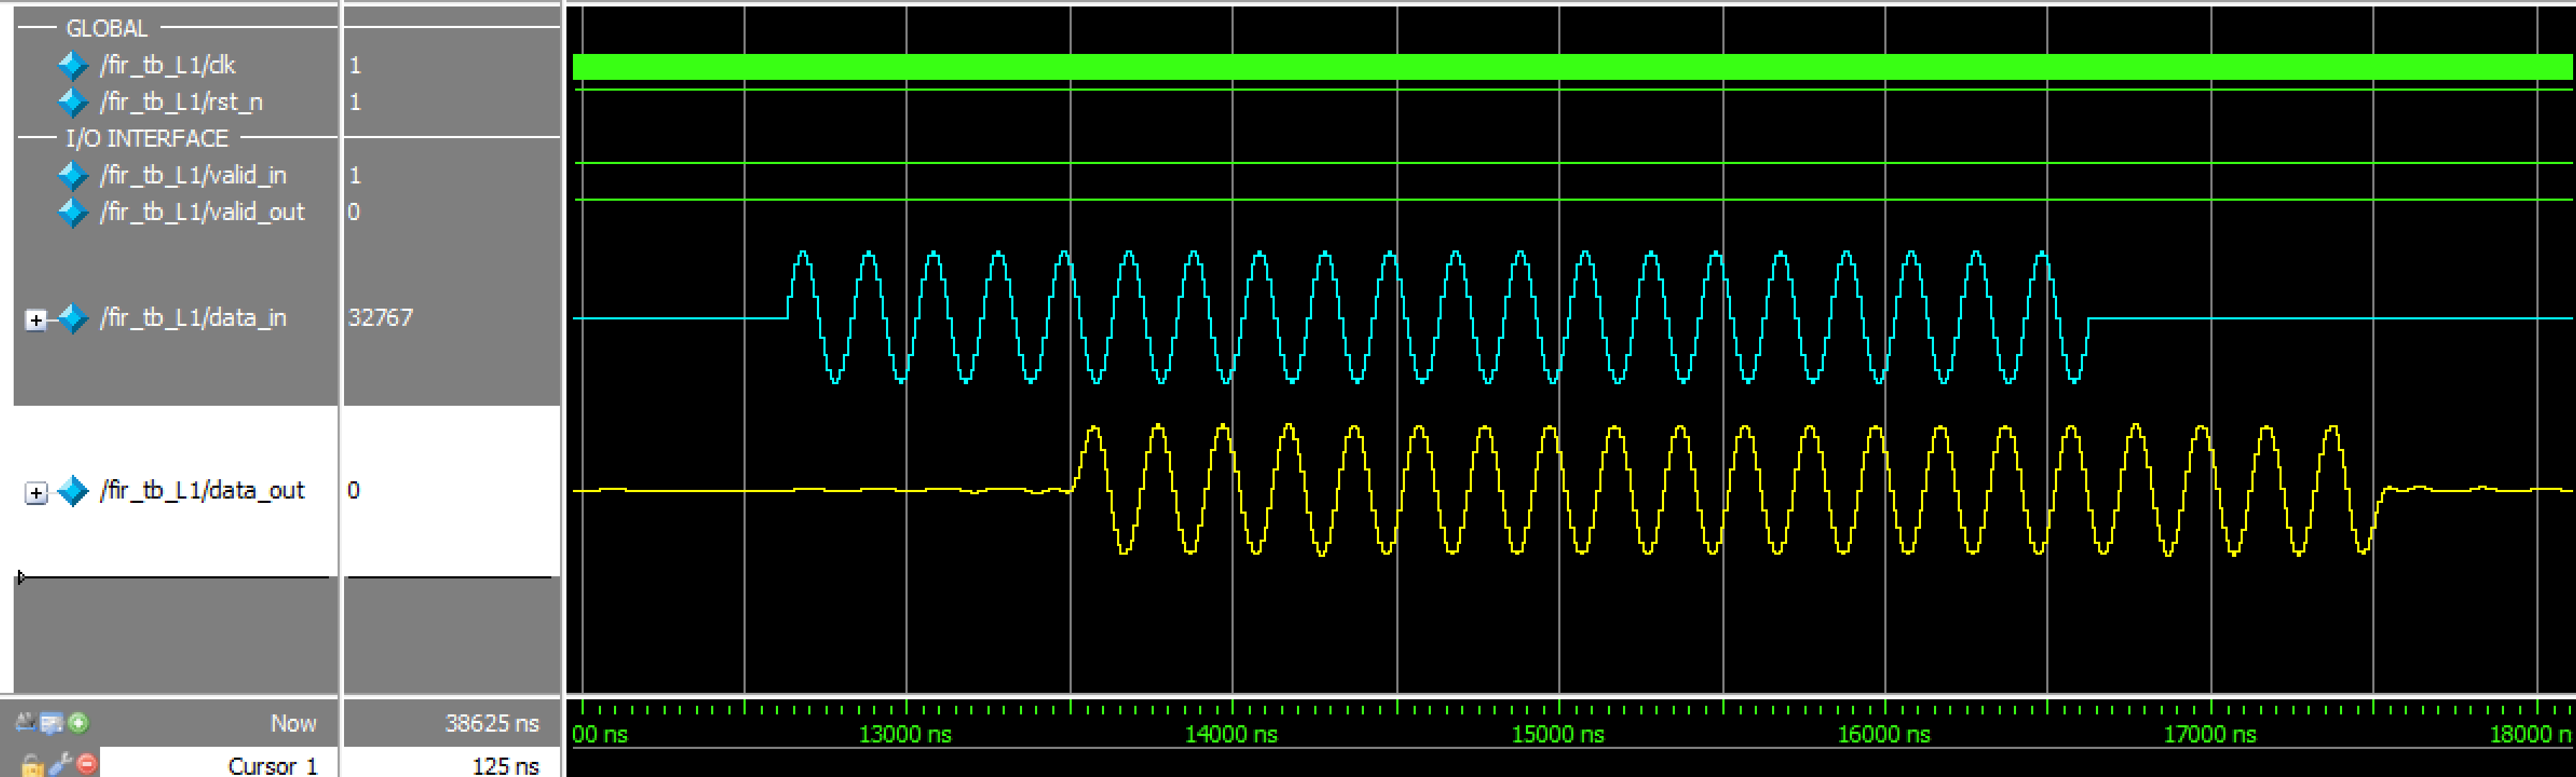
\includegraphics[width=0.95\linewidth]{images/waveforms/direct/low.png}
    \caption{Low Frequency: Direct Form.}
\end{figure}
\subsubsection{Pipelined FIR}
Confirm the passband signal matches the reference, following the expected pipeline delay.
\begin{figure}[H]
    \centering
    
\includegraphics[width=0.95\linewidth]{images/waveforms/pipelined/low.png}
    \caption{Low Frequency: Pipelined FIR.}
\end{figure}
\subsubsection{Parallel L=2}
Observe the low-frequency signal components as seen across the two parallel lanes.
\begin{figure}[H]
    \centering
    
\includegraphics[width=0.95\linewidth]{images/waveforms/parallel2/low.png}
    \caption{Low Frequency: Parallel L=2.}
\end{figure}
\subsubsection{Fast FIR L=2}
Verify the gain and phase response for a low-frequency stimulus in the Fast FIR design.
\begin{figure}[H]
    \centering
    
\includegraphics[width=0.95\linewidth]{images/waveforms/fast2/low.png}
    \caption{Low Frequency: Fast FIR L=2.}
\end{figure}
\subsubsection{Parallel L=3}
Observe the low-frequency signal distribution in the $L=3$ parallel architecture.
\begin{figure}[H]
    \centering
    
\includegraphics[width=0.95\linewidth]{images/waveforms/parallel3/low.png}
    \caption{Low Frequency: Parallel L=3.}
\end{figure}
\subsubsection{Fast FIR L=3}
Confirm that the passband signal is correctly processed by the $L=3$ Fast FIR algorithm.
\begin{figure}[H]
    \centering
    
\includegraphics[width=0.95\linewidth]{images/waveforms/fast3/low.png}
    \caption{Low Frequency: Fast FIR L=3.}
\end{figure}
\subsubsection{Pipelined Fast FIR L=3}
Note the processed passband signal at the full throughput of three samples per cycle.
\begin{figure}[H]
    \centering
    
\includegraphics[width=0.95\linewidth]{images/waveforms/fastpipe3/low.png}
    \caption{Low Frequency: Pipelined Fast FIR L=3.}
\end{figure}

\subsection{High Frequency}
\subsubsection{Direct Form}
Note the high degree of stopband attenuation for this high-frequency stimulus.
\begin{figure}[H]
    \centering
    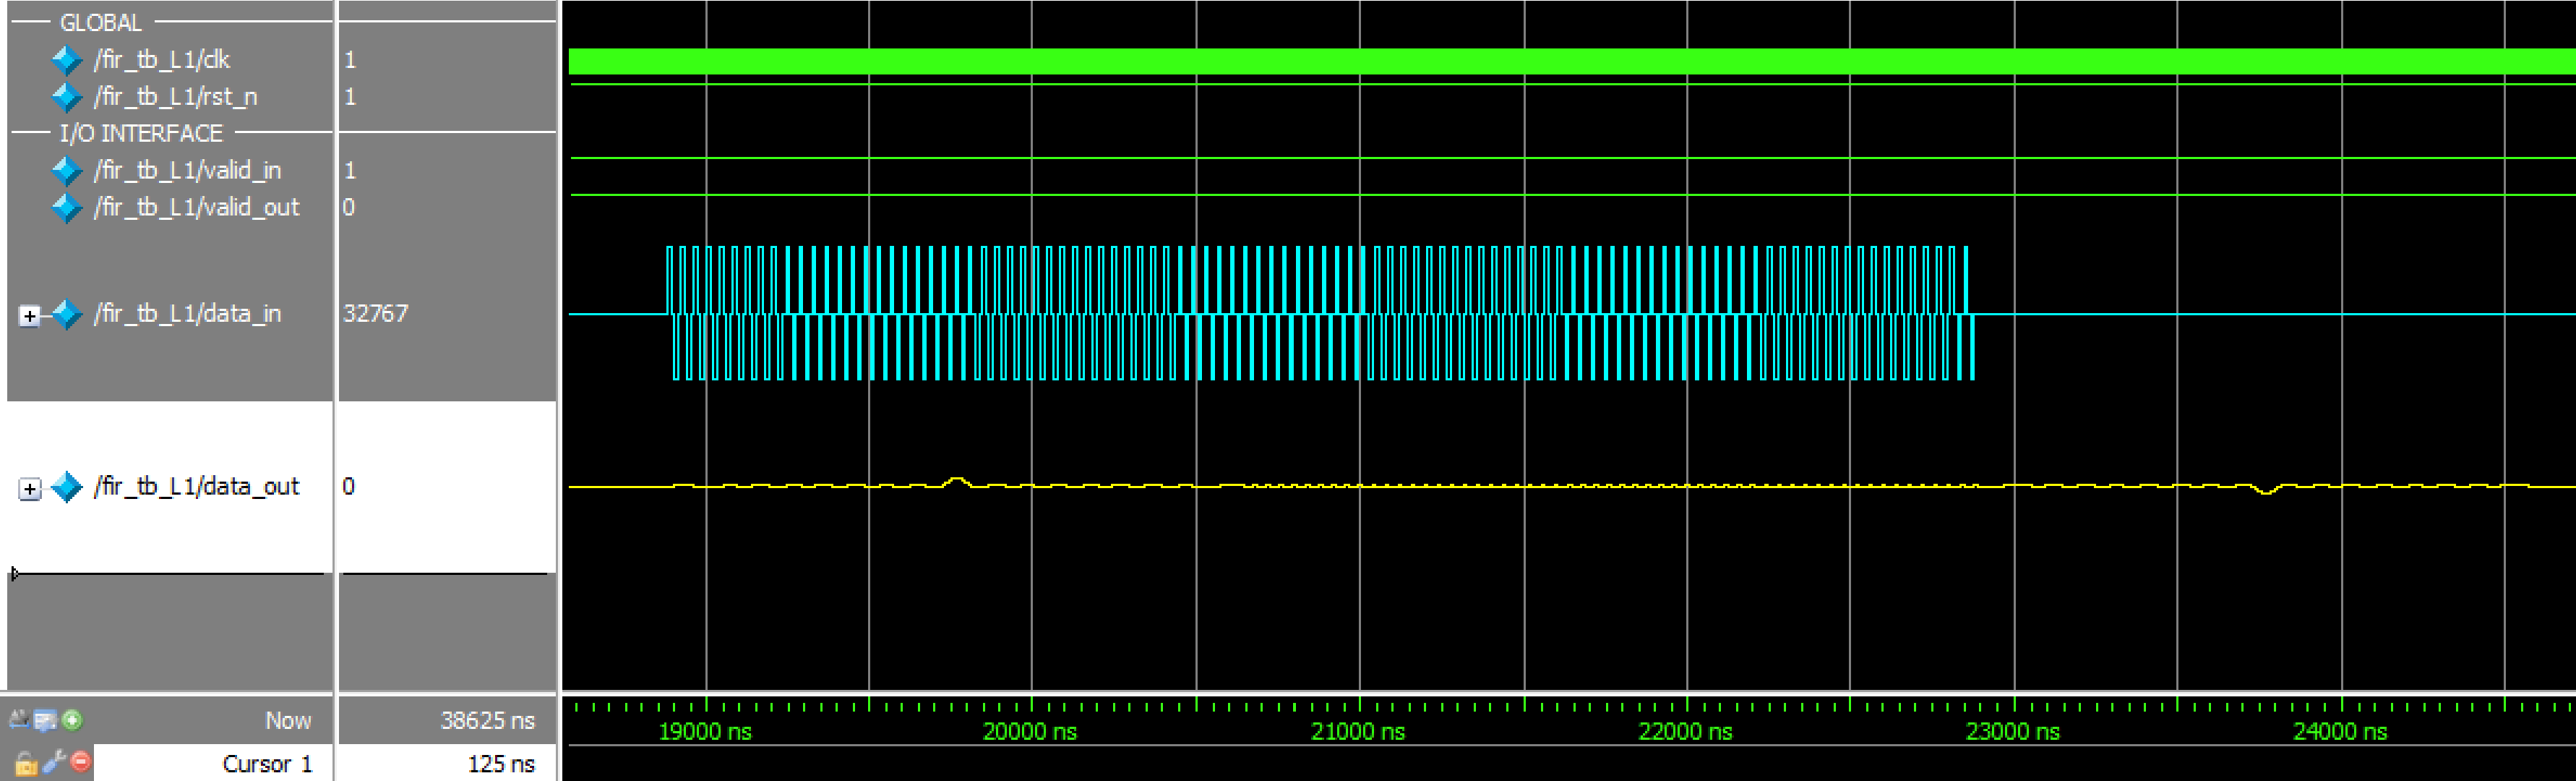
\includegraphics[width=0.95\linewidth]{images/waveforms/direct/high.png}
    \caption{High Frequency: Direct Form.}
\end{figure}
\subsubsection{Pipelined FIR}
Verify the effective rejection of high-frequency components by the pipelined filter.
\begin{figure}[H]
    \centering
    
\includegraphics[width=0.95\linewidth]{images/waveforms/pipelined/high.png}
    \caption{High Frequency: Pipelined FIR.}
\end{figure}
\subsubsection{Parallel L=2}
Observe the suppressed high-frequency signal across the parallel processing lanes.
\begin{figure}[H]
    \centering
    
\includegraphics[width=0.95\linewidth]{images/waveforms/parallel2/high.png}
    \caption{High Frequency: Parallel L=2.}
\end{figure}
\subsubsection{Fast FIR L=2}
Confirm the stopband rejection performance for the Fast FIR L=2 design.
\begin{figure}[H]
    \centering
    
\includegraphics[width=0.95\linewidth]{images/waveforms/fast2/high.png}
    \caption{High Frequency: Fast FIR L=2.}
\end{figure}
\subsubsection{Parallel L=3}
Verify the rejection of high-frequency noise in the $L=3$ parallel implementation.
\begin{figure}[H]
    \centering
    
\includegraphics[width=0.95\linewidth]{images/waveforms/parallel3/high.png}
    \caption{High Frequency: Parallel L=3.}
\end{figure}
\subsubsection{Fast FIR L=3}
Note the near-zero output levels, validating the $>$80 dB stopband attenuation.
\begin{figure}[H]
    \centering
    
\includegraphics[width=0.95\linewidth]{images/waveforms/fast3/high.png}
    \caption{High Frequency: Fast FIR L=3.}
\end{figure}
\subsubsection{Pipelined Fast FIR L=3}
Observe the high-frequency rejection at the peak architectural throughput.
\begin{figure}[H]
    \centering
    
\includegraphics[width=0.95\linewidth]{images/waveforms/fastpipe3/high.png}
    \caption{High Frequency: Pipelined Fast FIR L=3.}
\end{figure}

\subsection{Quantized Performance}
\subsubsection{Direct Form}
Confirm that the RTL output matches the 16-bit fixed-point quantized MATLAB model.
\begin{figure}[H]
    \centering
    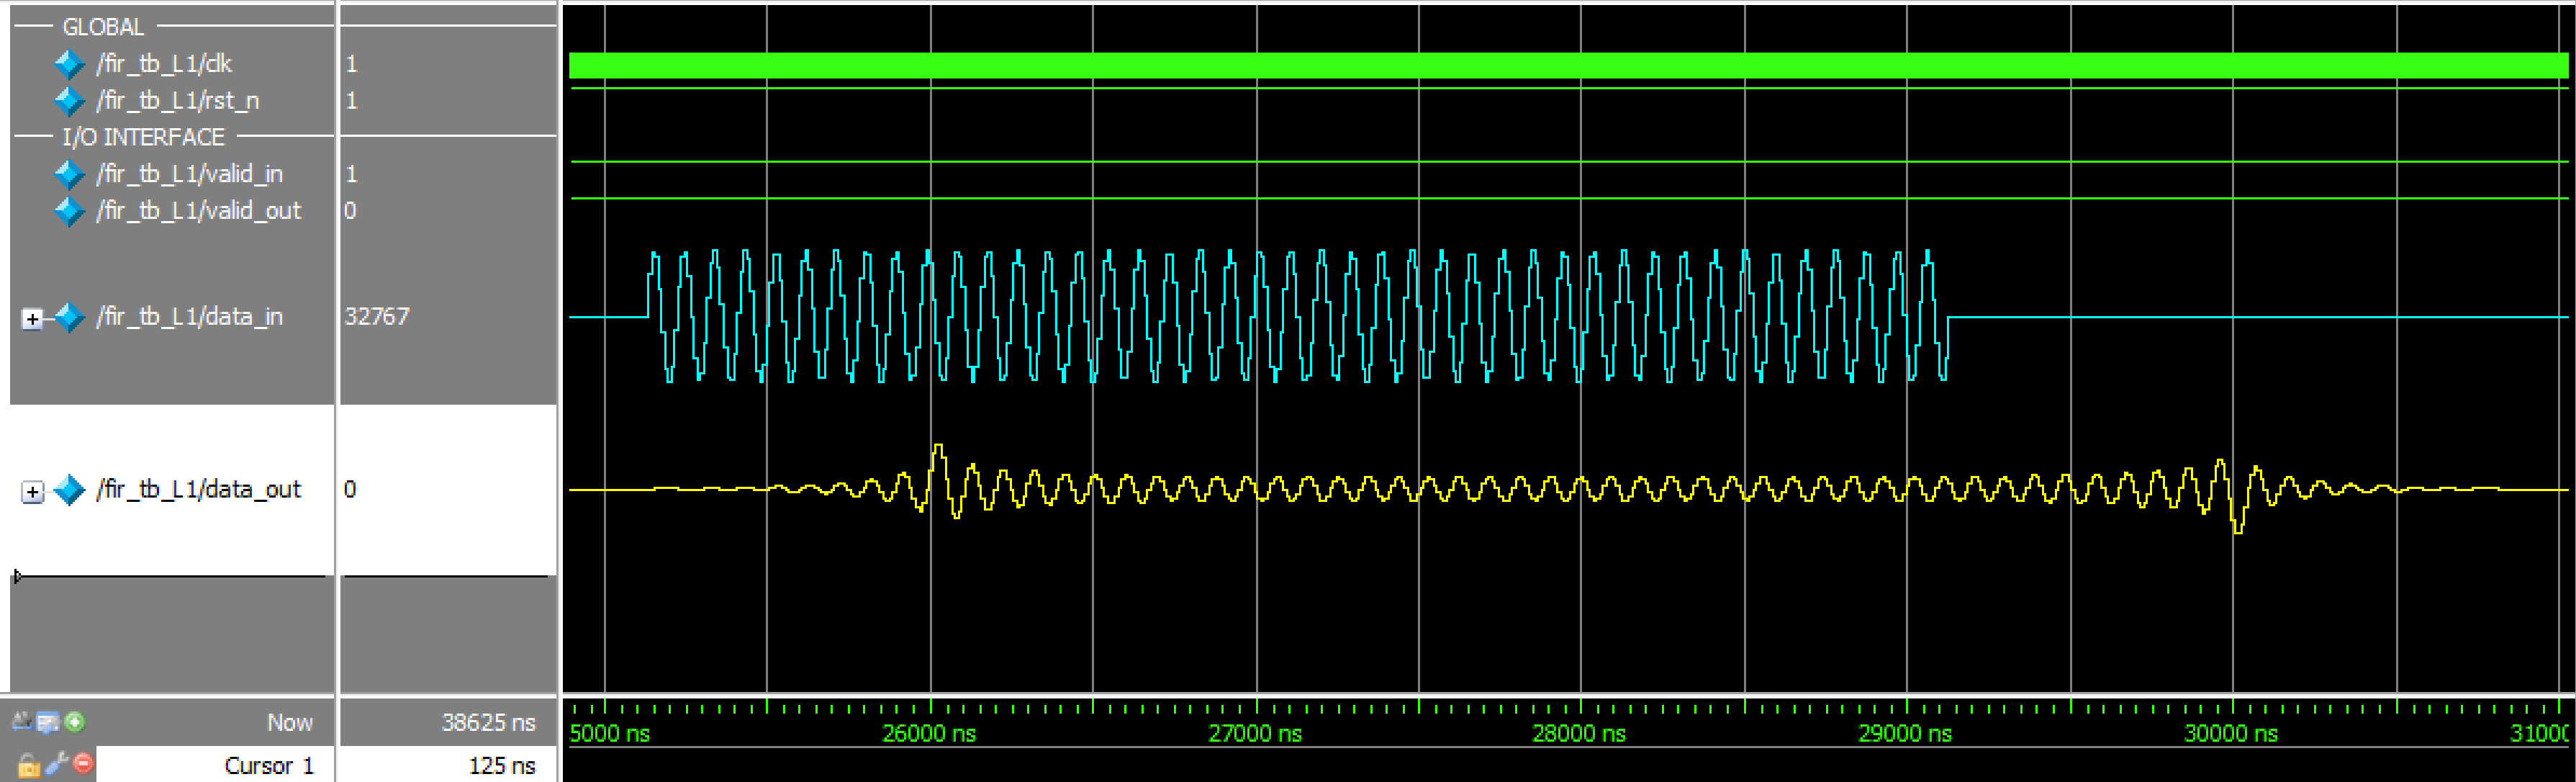
\includegraphics[width=0.95\linewidth]{images/waveforms/direct/quantized.png}
    \caption{Quantized Performance: Direct Form.}
\end{figure}
\subsubsection{Pipelined FIR}
Observe the quantization noise floor while verifying bit-exact matches with the golden model.
\begin{figure}[H]
    \centering
    
\includegraphics[width=0.95\linewidth]{images/waveforms/pipelined/quantized.png}
    \caption{Quantized Performance: Pipelined FIR.}
\end{figure}
\subsubsection{Parallel L=2}
Verify the quantized performance across the parallel polyphase sub-filters.
\begin{figure}[H]
    \centering
    
\includegraphics[width=0.95\linewidth]{images/waveforms/parallel2/quantized.png}
    \caption{Quantized Performance: Parallel L=2.}
\end{figure}
\subsubsection{Fast FIR L=2}
Confirm that the Fast FIR logic correctly handles the fixed-point quantization.
\begin{figure}[H]
    \centering
    
\includegraphics[width=0.95\linewidth]{images/waveforms/fast2/quantized.png}
    \caption{Quantized Performance: Fast FIR L=2.}
\end{figure}
\subsubsection{Parallel L=3}
Observe the quantized signal response for the $L=3$ parallel architecture.
\begin{figure}[H]
    \centering
    
\includegraphics[width=0.95\linewidth]{images/waveforms/parallel3/quantized.png}
    \caption{Quantized Performance: Parallel L=3.}
\end{figure}
\subsubsection{Fast FIR L=3}
Verify the bit-exact quantized match for the $L=3$ Fast FIR implementation.
\begin{figure}[H]
    \centering
    
\includegraphics[width=0.95\linewidth]{images/waveforms/fast3/quantized.png}
    \caption{Quantized Performance: Fast FIR L=3.}
\end{figure}
\subsubsection{Pipelined Fast FIR L=3}
Confirm high-fidelity processing for the optimized design under quantization.
\begin{figure}[H]
    \centering
    
\includegraphics[width=0.95\linewidth]{images/waveforms/fastpipe3/quantized.png}
    \caption{Quantized Performance: Pipelined Fast FIR L=3.}
\end{figure}

\subsection{Noisy Signal}
\subsubsection{Direct Form}
Observe the filter's ability to extract the signal from a noise-corrupted input.
\begin{figure}[H]
    \centering
    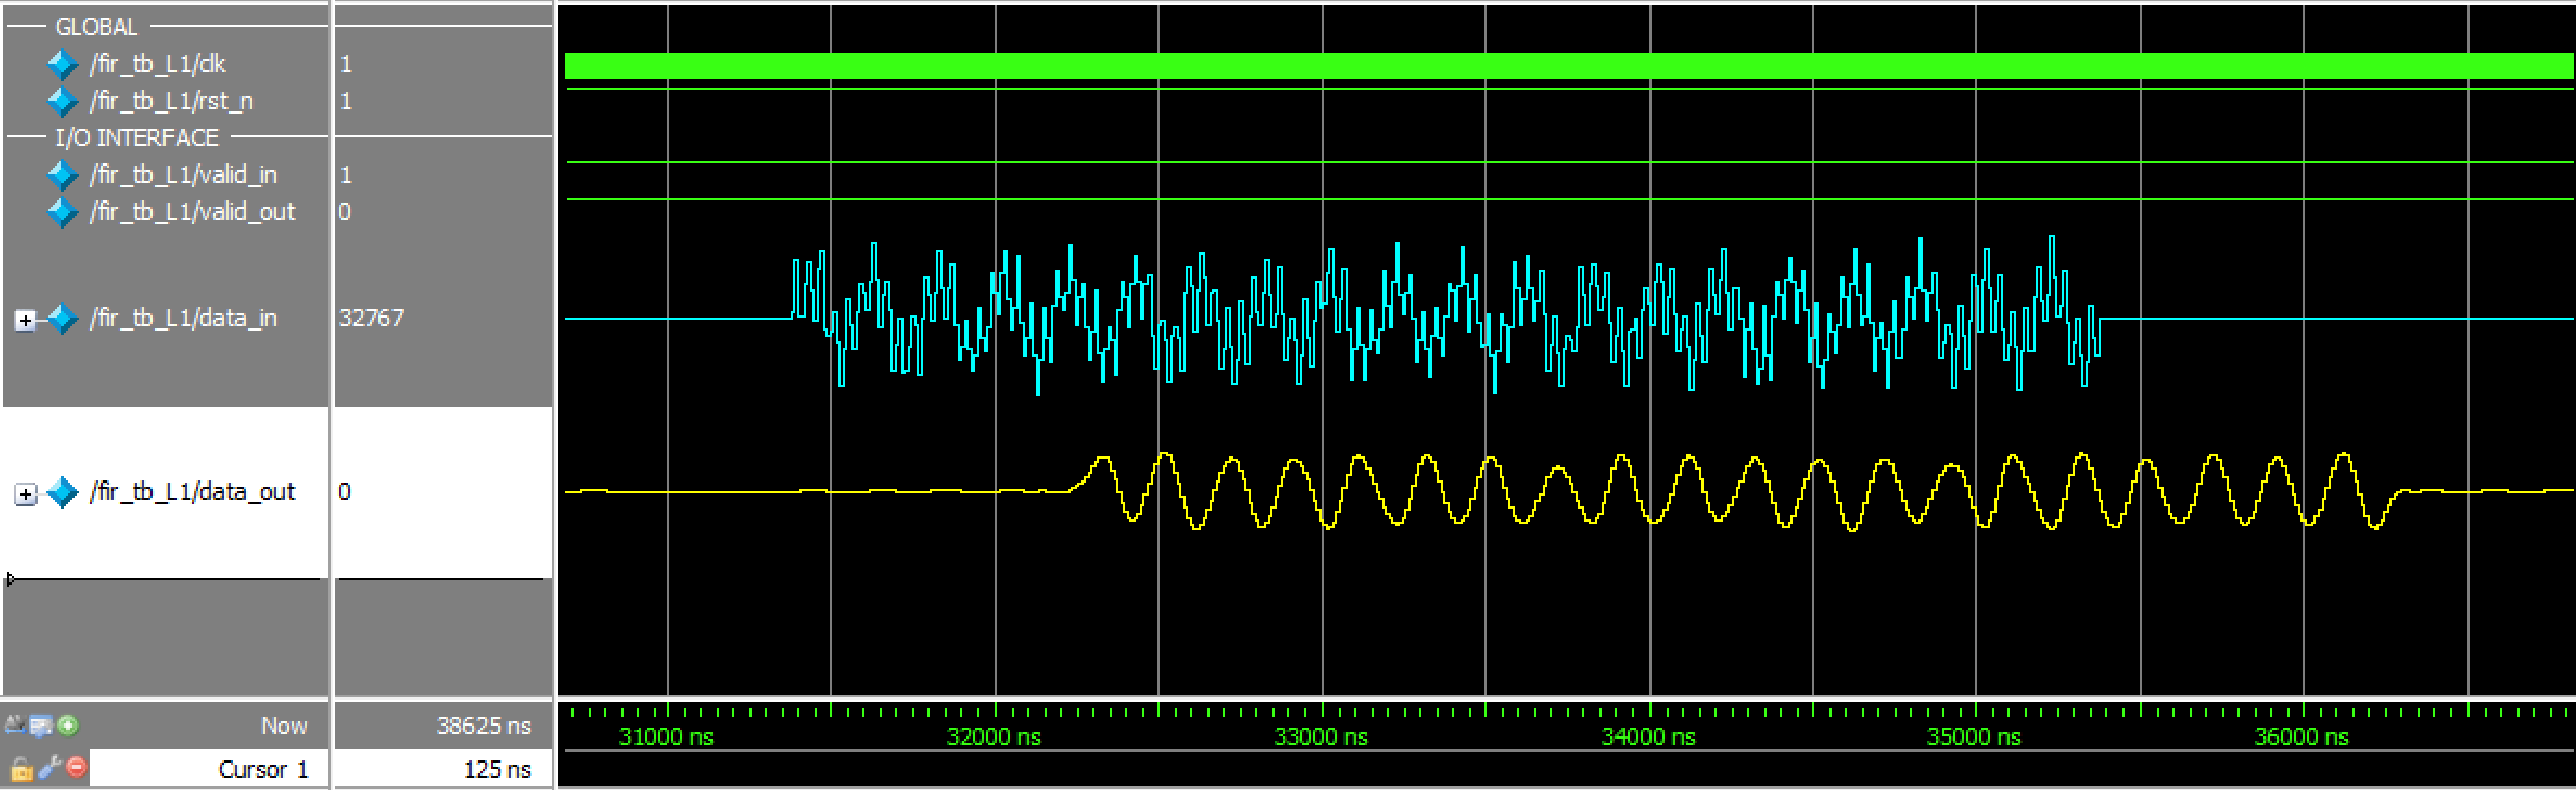
\includegraphics[width=0.95\linewidth]{images/waveforms/direct/noisy.png}
    \caption{Noisy Signal: Direct Form.}
\end{figure}
\subsubsection{Pipelined FIR}
Verify the successful rejection of high-frequency noise in the pipelined design.
\begin{figure}[H]
    \centering
    
\includegraphics[width=0.95\linewidth]{images/waveforms/pipelined/noisy.png}
    \caption{Noisy Signal: Pipelined FIR.}
\end{figure}
\subsubsection{Parallel L=2}
Note the noise reduction performance when processing data in parallel lanes.
\begin{figure}[H]
    \centering
    
\includegraphics[width=0.95\linewidth]{images/waveforms/parallel2/noisy.png}
    \caption{Noisy Signal: Parallel L=2.}
\end{figure}
\subsubsection{Fast FIR L=2}
Confirm the noise suppression capability of the Fast FIR L=2 architecture.
\begin{figure}[H]
    \centering
    
\includegraphics[width=0.95\linewidth]{images/waveforms/fast2/noisy.png}
    \caption{Noisy Signal: Fast FIR L=2.}
\end{figure}
\subsubsection{Parallel L=3}
Observe the smoothed output signal recovered from the noisy input at $L=3$.
\begin{figure}[H]
    \centering
    
\includegraphics[width=0.95\linewidth]{images/waveforms/parallel3/noisy.png}
    \caption{Noisy Signal: Parallel L=3.}
\end{figure}
\subsubsection{Fast FIR L=3}
Verify effective noise filtering for the $L=3$ Fast FIR sub-filter logic.
\begin{figure}[H]
    \centering
    
\includegraphics[width=0.95\linewidth]{images/waveforms/fast3/noisy.png}
    \caption{Noisy Signal: Fast FIR L=3.}
\end{figure}
\subsubsection{Pipelined Fast FIR L=3}
Confirm high-quality signal recovery at maximum throughput.
\begin{figure}[H]
    \centering
    
\includegraphics[width=0.95\linewidth]{images/waveforms/fastpipe3/noisy.png}
    \caption{Noisy Signal: Pipelined Fast FIR L=3.}
\end{figure}

\subsection{Pipeline Latency}
\subsubsection{Direct Form}
Measure the single-cycle delay from input stimulus to the first valid output sample.
\begin{figure}[H]
    \centering
    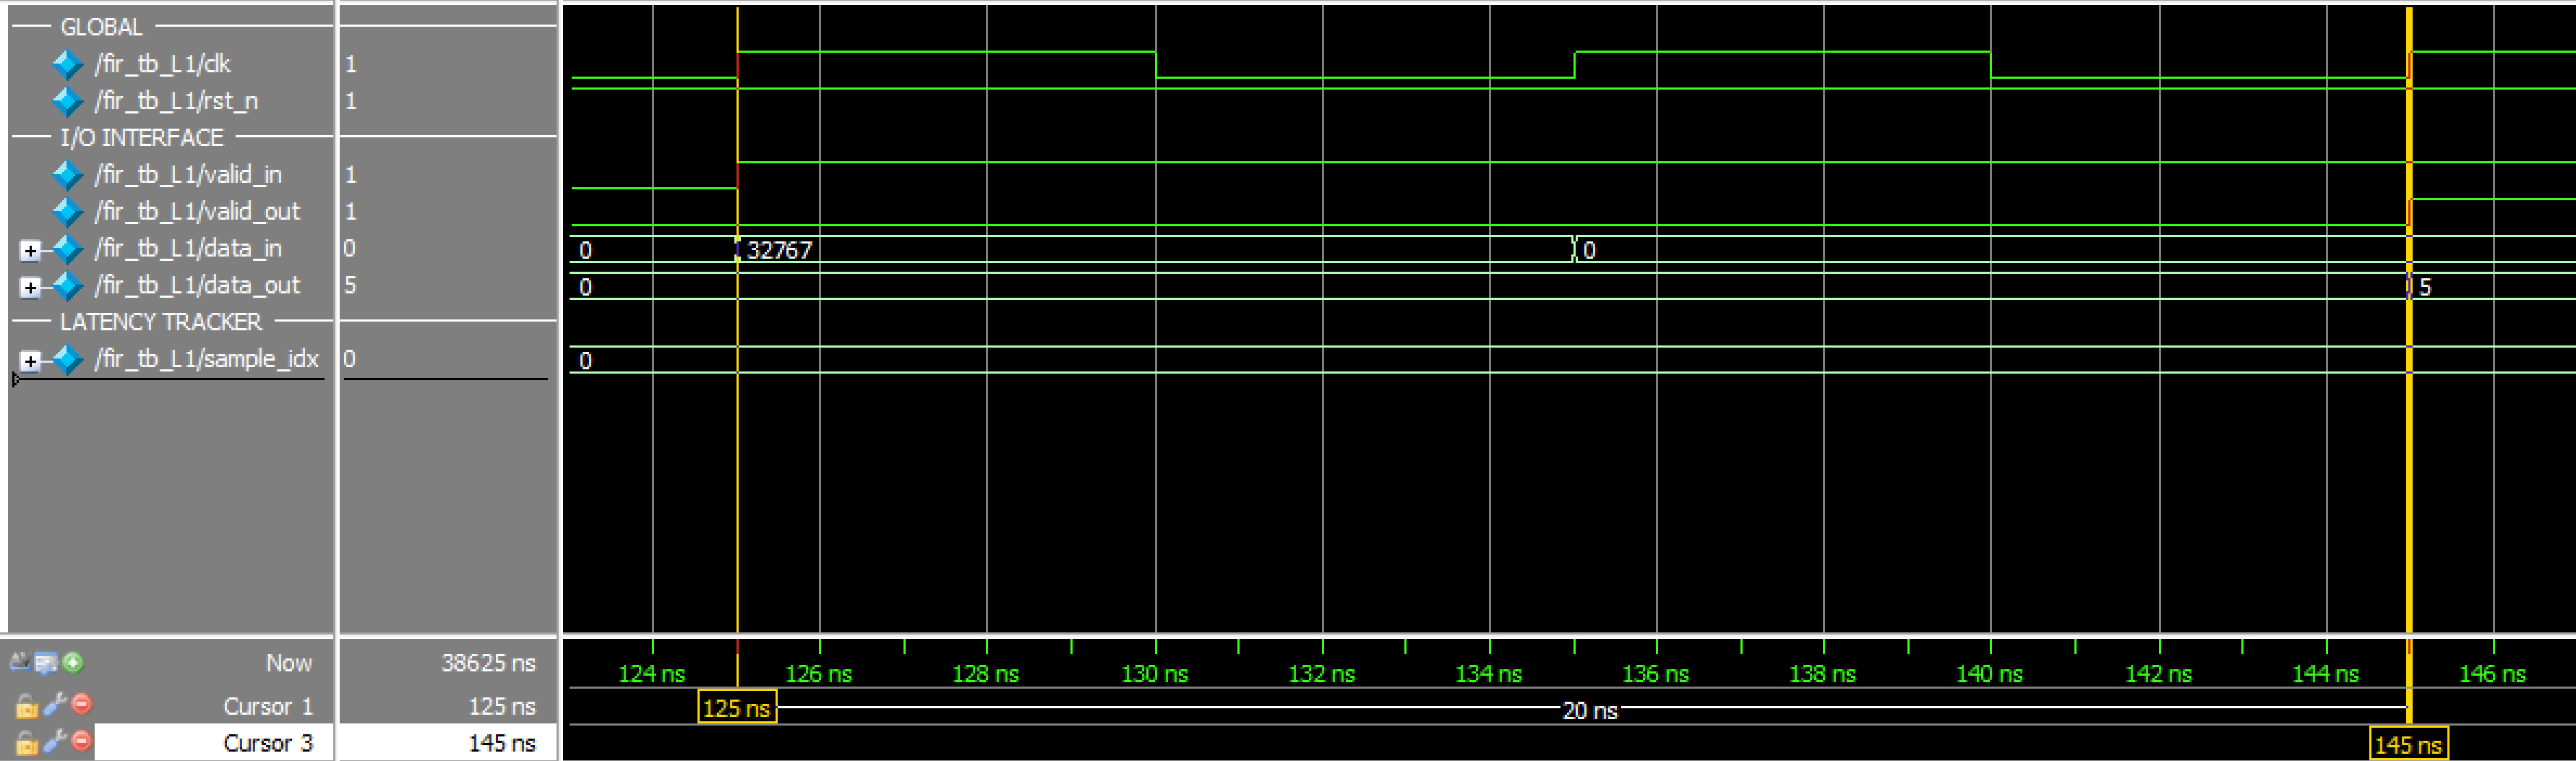
\includegraphics[width=0.95\linewidth]{images/waveforms/direct/latency.png}
    \caption{Pipeline Latency: Direct Form.}
\end{figure}
\subsubsection{Pipelined FIR}
Observe the additional cycles of latency introduced by the pipeline registers.
\begin{figure}[H]
    \centering
    
\includegraphics[width=0.95\linewidth]{images/waveforms/pipelined/latency.png}
    \caption{Pipeline Latency: Pipelined FIR.}
\end{figure}
\subsubsection{Parallel L=2}
Measure the latency from the first interleaved input to the valid parallel output.
\begin{figure}[H]
    \centering
    
\includegraphics[width=0.95\linewidth]{images/waveforms/parallel2/latency.png}
    \caption{Pipeline Latency: Parallel L=2.}
\end{figure}
\subsubsection{Fast FIR L=2}
Verify the specific delay characteristics of the Fast FIR L=2 processing path.
\begin{figure}[H]
    \centering
    
\includegraphics[width=0.95\linewidth]{images/waveforms/fast2/latency.png}
    \caption{Pipeline Latency: Fast FIR L=2.}
\end{figure}
\subsubsection{Parallel L=3}
Confirm the clock cycle delay for data traversing the $L=3$ parallel lanes.
\begin{figure}[H]
    \centering
    
\includegraphics[width=0.95\linewidth]{images/waveforms/parallel3/latency.png}
    \caption{Pipeline Latency: Parallel L=3.}
\end{figure}
\subsubsection{Fast FIR L=3}
Identify the processing latency for the $L=3$ Fast FIR sub-filter logic.
\begin{figure}[H]
    \centering
    
\includegraphics[width=0.95\linewidth]{images/waveforms/fast3/latency.png}
    \caption{Pipeline Latency: Fast FIR L=3.}
\end{figure}
\subsubsection{Pipelined Fast FIR L=3}
Measure the combined latency of the fast FIR logic and the internal pipeline stages.
\begin{figure}[H]
    \centering
    
\includegraphics[width=0.95\linewidth]{images/waveforms/fastpipe3/latency.png}
    \caption{Pipeline Latency: Pipelined Fast FIR L=3.}
\end{figure}

\nocite{*}
\bibliographystyle{plain}
\bibliography{references}

\end{document}
